\documentclass[12pt]{article}

% PLOS ONE formatting
\usepackage[margin=1in]{geometry}
\usepackage{fontspec}
\setmainfont{TeX Gyre Termes}  % Times New Roman equivalent
\usepackage{unicode-math}
\usepackage{setspace}
\doublespacing
\usepackage{lineno}
\linenumbers
\usepackage{amsmath}
\usepackage{booktabs}
\usepackage{longtable}
\usepackage{tabularx}
\usepackage{graphicx}
\usepackage{hyperref}
\hypersetup{colorlinks=true,linkcolor=black,citecolor=black,urlcolor=blue}
\usepackage{microtype}

% Fix longtable + doublespacing interaction
\usepackage{etoolbox}
\AtBeginEnvironment{longtable}{\singlespacing\small}

% No paragraph indent, use skip instead
\setlength{\parindent}{0pt}
\setlength{\parskip}{6pt plus 2pt minus 1pt}

% Section formatting - numbered
\usepackage{titlesec}
\titleformat{\section}{\normalfont\large\bfseries}{\thesection.}{0.5em}{}
\titleformat{\subsection}{\normalfont\normalsize\bfseries}{\thesubsection}{0.5em}{}
\titleformat{\subsubsection}{\normalfont\normalsize\itshape}{\thesubsubsection}{0.5em}{}

% Page numbers
\usepackage{fancyhdr}
\pagestyle{fancy}
\fancyhf{}
\fancyfoot[C]{\thepage}
\renewcommand{\headrulewidth}{0pt}

% Caption formatting
% caption formatting handled by default



\begin{document}

% ============================================================
% TITLE PAGE
% ============================================================
\begin{center}
{\Large\bfseries Code Geometry and Endogenous Enforcement Concentration\\
in an Agent-Based Model of Fundamentalism}

\bigskip

{[Author Name]}

{[Affiliation]}

{[Corresponding author email]}
\end{center}

%
\section*{Abstract}

Enforcement-dominant dynamics in codified moral systems arise from
structural properties of the code, not from the content of belief or the
psychology of believers. An agent-based model with symmetric agents
($N = 350$; no pre-assigned enforcement roles; approximately 5,000 runs
across eight experimental specifications) demonstrates a monotonic,
threshold-gated relationship between code legibility and enforcement
regime. A fine-grained dose-response sweep (1,200 runs across ten
legibility values) identifies a critical transition whose position
depends on enforcement reward: at moderate reward ($\pi = 0.25$), the
boundary lies near $\sigma \approx 0.3$; at high reward ($\pi = 0.50$),
it shifts to $\sigma \approx 0.2$. Below this boundary, enforcement
cannot activate regardless of other parameters. Above it, institutional
delegation concentrates punishment in an endogenously selected minority
and narrative drift collapses exit (median exit rate 0.08). Ablation
confirms that concentration is genuinely endogenous: removing the
institutional monopoly restriction leaves concentration metrics
unchanged (top-5 share: 0.81--0.90 in both conditions; $n = 180$
matched runs). Two theoretically motivated retention
mechanisms--sanctified suffering and membership reward--are inert
across their full parameter ranges. Only endogenous degradation of the
perceived outside option converts enforcement concentration into durable
capture. Cross-national analysis ($N = 36$ countries) indicates that
both outside-option quality and enforcement legislation independently
predict religious retention in a combined model ($R^2 = 0.73$); the
analysis is exploratory and underpowered to rank their relative
contributions. Legibility is the gate; enforcement reward shifts
the boundary; endogenous narrative drift closes the trap.

\section{Introduction}

When religious fundamentalism is discussed as a social problem, the standard causal story runs through actors: extremists capture institutions, radicalize communities, and impose orthodoxy on reluctant majorities. The prescription follows naturally: identify and neutralize the extremists, and the system returns to health. This framing treats enforcement specialists as exogenous to the belief system, a pathogen that could in principle be removed without altering the host.

The present paper argues that this framing is structurally incomplete. We propose that enforcement-dominant dynamics (the behavioral syndrome typically labeled "fundamentalism") are better understood as an endogenous equilibrium of codified moral systems with specific structural properties. The key structural variable is not theological content but what we term \emph{code geometry}: the configuration of a moral code's legibility (the degree to which compliance is externally observable), substitutability (the degree to which external performance can replace internal transformation as a criterion of moral standing), enforcement affordance (the ease with which deviations can be detected and sanctioned), centralization of adjudication, and exit cost. We show, using an agent-based model parameterized by these five dimensions, that enforcement equilibria emerge without importing abnormal psychological distributions, charismatic leadership, or exogenous political shocks. The model generates four distinct regime types (quiet, mixed enforcement, collapse, and capture) whose boundaries are determined by code geometry rather than by the beliefs held within the system.

The central empirical prediction is that codified moral systems scoring high on legibility, substitutability, and enforcement affordance will generate enforcement-specialist niches regardless of the specific doctrinal commitments involved. This prediction is domain-general: it applies to religious traditions, secular ideologies with purity requirements, and any identity-bearing system that codifies behavioral expectations and makes compliance a condition of standing. Religion provides the most historically developed and best-documented instances, and we draw on religious cases throughout, but the mechanism does not depend on supernatural content.

Three features of this framework distinguish it from existing accounts. First, legibility is formalized as a continuous parameter of code structure, an information-theoretic property, rather than as a cost to the agent (as in costly signaling theory) or a behavioral demand (as in club-goods models of strictness). This draws on James C. Scott's concept of state legibility but extends it, for the first time in formal modeling, to belief enforcement. Second, the model derives four qualitatively distinct regimes from the interaction of code geometry parameters, whereas existing frameworks typically produce binary outcomes (cooperation vs. defection, exit vs. voice, strict vs. lenient). Third, the model demonstrates that minority enforcement capture requires institutional delegation and compounding enforcement capital, not merely preference asymmetry among agents, a prediction that directly contradicts the intolerant-minority mechanism proposed by Taleb[40] and the committed-minority models of opinion dynamics.


A structural observation motivates the dose-response analysis reported in
\S8.12. The legibility parameter $\sigma$ corresponds to a deep
architectural feature of codified systems: the degree to which the
system's authority structure renders moral compliance externally
auditable. Systems that locate authority in transpersonal principles
structurally resist legibility, because the compliance that
matters--internal realization, contemplative attainment--is opaque to
observers. Systems that locate authority in person-dependent revelation
structurally produce legibility, because the compliance that
matters--behavioral adherence to codified prescriptions--is externally
visible and binary. The model tests whether this architectural
difference, formalized as $\sigma$, determines enforcement regime. It
does, but not alone: $\sigma$ gates activation, $\pi$ shifts the
activation boundary, and endogenous $\delta$ drift determines whether
activation produces transient enforcement or durable capture.

The paper proceeds as follows. Section 2 reviews existing literature organized by mechanism rather than by discipline, identifies the specific theoretical gap, and locates the contribution relative to rational-choice sociology of religion, evolutionary game theory, new institutionalism, and political economy. Section 3 defines the code geometry framework. Section 4 provides the parameter-to-observable mapping. Section 5 presents the scoring rubric and falsifiability conditions. Section 6 specifies the agent-based model: population structure, agent decision rules, enforcement mechanics, exit dynamics, and the endogenous narrative drift mechanism. Section 7 addresses scope and limitations. Section 8 presents results: regime phase diagrams, ablation studies isolating the causal mechanism, and punishment concentration metrics. Section 9 discusses historical anchoring, empirical predictions, relationship to existing frameworks, and falsifiability. Section 10 states the conclusions.

%
\section{Literature Positioning}

%
\subsection{Enforcement and strictness in the rational-choice tradition}

The dominant formal framework for understanding why high-cost religious groups persist and grow is the club-goods model developed by Iannaccone [23,24]. In this framework, costly behavioral demands (dietary restrictions, dress codes, tithing, time-intensive rituals) function as screening mechanisms that exclude free-riders, raising the average quality of participation and the value of club goods (mutual aid, social capital, communal identity). Strictness is the price of admission; groups that charge higher prices attract more committed members and outcompete lenient groups in cohesion and mobilization.

This framework captures an important mechanism, and the empirical pattern it explains (that strict denominations grow while lenient ones decline) is robust. But it leaves three questions unanswered that are central to the phenomenon of enforcement-dominant dynamics. First, enforcement in the club model operates through screening (an ex ante mechanism): costly demands filter the population before entry. The model does not address ex post enforcement: the active policing, sanctioning, and punishment of members who have already joined. The transition from "strict requirements attract committed members" to "enforcement specialists police the community" is not formalized. Second, the club model does not produce a structural distinction between moderate strictness (functional screening) and enforcement dominance (coercive control by a specialized minority). These are treated as points on a continuum rather than as qualitatively different regimes. Iannaccone[24] acknowledged that excessive strictness can backfire: "a church reaches [the tipping] point when it fails to offer acceptable substitutes for everything it has asked its members to give up," but the tipping point is not modeled as a regime transition. Third, the club model assumes voluntary participation. Members choose the strict bundle; those who dislike it leave. This assumption is reasonable for denominational choice in pluralistic religious markets but fails in contexts where exit is blocked, where apostasy carries legal penalties, kinship networks are wholly internal, or economic livelihood depends on community membership.

Berman[3] extended the club framework to ultra-Orthodox Jewish communities, where yeshiva attendance creates non-transferable religious human capital that functions as a powerful exit cost. Berman and Laitin[4] applied similar logic to terrorist organizations, where sacrifice requirements solve principal-agent problems in covert operations. Carvalho[7] formalized veiling as a commitment mechanism with implicit reputational costs for non-compliance. These extensions move closer to the dynamics of enforcement (Berman's religious capital is the strongest existing formalization of exit cost as a lock-in device), but none introduces positive enforcement payoffs to sanctioners, institutional delegation of punishment authority, or the compounding of enforcement capacity over time. The gap is consistent: the club tradition explains why strict groups can be stable but does not explain how enforcement authority concentrates in a minority or how enforcement regimes become self-reinforcing.

%
\subsection{Punishment, monitoring, and the observability problem}

A parallel literature in evolutionary game theory addresses the conditions under which punishment can stabilize cooperation. Boyd, Gintis, Bowles, and Richerson [5] demonstrated that altruistic punishment can evolve in large groups because punishment costs decrease as punishers become common. Fehr and Gächter [12,13] provided experimental evidence that costly punishment sustains cooperation and that cooperation collapses when punishment is unavailable. Axelrod[2] showed that metanorms (punishing those who fail to punish) can stabilize norm enforcement through second-order sanctioning.

These results establish that enforcement equilibria are achievable under general conditions. But a structural feature unites these models: punishment is treated as a \emph{cost} to the enforcer. Punishment is altruistic; it benefits the group at the expense of the individual punisher. This is a reasonable assumption for many settings, but it does not describe the dynamics of institutionalized enforcement in codified belief systems, where enforcers routinely gain status, institutional access, and material rewards for policing. Clerical promotion contingent on orthodoxy enforcement, social prestige for public correction of deviants, and institutional budgets tied to enforcement activity all represent \emph{positive} payoffs to sanctioners. When enforcement is profitable rather than costly, the dynamics change qualitatively: enforcement becomes self-sustaining not because punishers are altruistic but because the enforcement niche is structurally rewarding.

The closest formal predecessor to this dynamic is Centola, Willer, and Macy's [8] Emperor's Dilemma, an agent-based model where cascades of support for unpopular norms emerge when enforcement is observable and enforcers gain status. A small minority of "true believers" can induce majority compliance through self-reinforcing enforcement cascades. This model captures the core intuition (that enforcement can spread as a social strategy even without genuine belief), but it treats compliance as binary, does not model exit, and does not introduce institutional delegation or compounding enforcement capacity. The cascade operates through decentralized peer pressure rather than through a specialized enforcement apparatus.

A second structural limitation of the punishment literature is the treatment of observability. Punishment requires that defection (or noncompliance) be observable. This observation-dependence is implicit in nearly all punishment models but is rarely formalized as a variable property of the system being enforced. The degree to which a moral code renders compliance observable is not a constant; it is a design feature of the code itself. A code that demands observable acts (attend Friday prayers, wear prescribed clothing, observe dietary restrictions publicly) generates fundamentally different enforcement dynamics than a code that demands internal states (reduce anger, cultivate compassion, attain non-attachment). Scott[37] developed this insight at length for state governance (standardization and simplification render populations legible to administrative control), but no formal model has applied Scott's legibility concept to belief enforcement. This gap is the origin of our σ parameter.

%
\subsection{Exit, voice, and the regime problem}

Hirschman's [21] Exit, Voice, and Loyalty provides the canonical framework for organizational responses to decline: members can leave (exit), attempt reform (voice), or remain despite dissatisfaction (loyalty). Hirschman noted that religions explicitly position themselves as unsubstitutable, thereby raising loyalty and suppressing both exit and voice. The framework is structurally binary (exit or voice, modulated by loyalty) and does not distinguish between the qualitatively different outcomes that exit cost variation produces.

When exit is cheap and enforcement escalates, the expected outcome is fragmentation: dissatisfied members leave, the population contracts, and the enforcement apparatus loses targets. When exit is expensive and enforcement escalates, the expected outcome is very different: dissatisfied members are trapped, dissent is internalized, and enforcement can stabilize without corrective feedback from departures. These are not points on a continuum; they are distinct dynamical regimes with different attractor structures.

Kuran's [28] theory of preference falsification comes closest to formalizing this distinction. Citizens publicly express preferences differing from private beliefs under social pressure, producing "collective conservatism" (stable falsification) or "revolutionary cascades" (sudden dissolution when the falsification threshold breaks). Kuran discussed religious preference falsification explicitly (crypto-Judaism under the Inquisition, Shia \emph{taqiyya}) and his two-regime structure maps partially onto the collapse and mixed-enforcement regimes in our framework. However, Kuran does not formalize hierarchical capture as a distinct stable equilibrium. For him, all falsification equilibria are potentially unstable, subject to revolutionary cascade. The possibility that an enforcement-dominant minority can stabilize the system indefinitely through institutional delegation and compounding enforcement capital, preventing cascade even when private dissent is near-universal, is outside his framework.

The leaving-religion literature [6,11,39] provides extensive empirical documentation of exit costs and their consequences, but this scholarship is primarily descriptive and case-based. It does not formalize how exit cost interacts with enforcement parameters to generate distinct regime types. Agent-based models of secularization [16,30] model affiliation and disaffiliation dynamics but typically drive these through existential security or cognitive variables rather than enforcement geometry.

%
\subsection{Delegation, monopoly, and the missing mechanism of minority capture}

The theoretical gap that motivates this paper sits at the intersection of three well-developed literatures that have not been formally integrated.

State-formation theory provides the vocabulary of coercive monopoly. Weber [45] defined the state by its successful claim to monopoly over legitimate force. Tilly[41] described state-making as organized coercion with a ratcheting dynamic: war requires taxation, taxation requires administrative capacity, administrative capacity enables more war. Mann[29] distinguished despotic power (command) from infrastructural power (the capacity to penetrate society with rules and monitoring). These frameworks describe compounding coercive capacity at the macro-political level but have rarely been applied to the internal governance of belief systems.

New institutionalism provides the theory of enforcement equilibria and path dependence. North[31] defined institutions as formal and informal constraints plus enforcement characteristics, and noted that "formal rules are created to serve the interests of those with the bargaining power to create new rules": minority capture by institutional design. Greif[18] analyzed the transition from distributed to specialized enforcement in merchant communities. Greif and Mokyr[19] observed that "the fact that such an agent has been asked to legitimize a ruler is a source of additional power to such agents," a description of compounding enforcement capital that remains unformal. Pierson[32] formalized path dependence as an increasing-returns dynamic where early institutional advantages compound over time.

Political economy of religion provides case studies of enforcement delegation. Rubin[35] analyzed religious authorities as "legitimizing agents" who sit at the political bargaining table; Ottoman ulama monopolized religious scholarship and commercial law interpretation for centuries. Cook[10] traced the Islamic \emph{hisbah} doctrine from individual Muslim obligation to institutional enforcement apparatus. Given[17] documented how the medieval Inquisition accumulated records, informers, and procedural knowledge that compounded its enforcement capability across decades. Kelly[25] described the transition from personal inquisitorial authority to institutional jurisdiction, the shift from distributed to delegated enforcement.

Each of these literatures contains ingredients of the mechanism we formalize: coercive monopoly, enforcement delegation, compounding capacity, path dependence. But they have not been combined into a unified micro-level model that derives enforcement regimes from the interaction of code structure and institutional design. Evolutionary game theory has partially filled this gap through the distinction between peer punishment and pool punishment [20,38], showing that delegated institutional punishment produces qualitatively different equilibria than distributed individual punishment. But pool-punishment models treat the institution as solving the second-order punishment problem (who punishes non-punishers?), not as enabling minority capture of doctrinal authority through compounding enforcement capital.

%
\subsection{The gap}

No existing formal model combines the following five components: (1) legibility of moral compliance as a continuous structural parameter of the code, distinct from signaling cost; (2) positive enforcement payoffs to sanctioners, generating a self-sustaining enforcement niche; (3) exit cost as a regime determinant that distinguishes collapse from capture; (4) institutional delegation of punishment authority, concentrating enforcement in a minority; and (5) compounding enforcement capital that creates path-dependent power accumulation in the enforcement apparatus.

Each component has strong antecedents. Iannaccone formalized costly demands; Boyd et al.~formalized punishment dynamics; Berman formalized exit costs; Weber [45] and Tilly [41] described coercive monopoly; Greif and Pierson described path dependence. The synthesis is what generates the novel predictions: four qualitatively distinct regime types rather than binary outcomes, endogenous minority capture from enforcement geometry rather than from preference asymmetry, and the formal separation of enforcement intensity from belief prevalence, a divergence that existing models do not produce but that is empirically well-documented [9,42,43].

The contribution of this paper is to build that synthesis as a working computational model, demonstrate its regime structure, identify the causal mechanism through ablation, and provide a falsifiable scoring rubric for empirical evaluation.

%
\section{Theoretical Framework}

%
\subsection{Codified Moral Systems}

A codified moral system is a socially shared normative structure in which obligations, prohibitions, and membership criteria are articulated in transmissible rule-form and maintained across generations through institutional mechanisms. Religious traditions are the most historically durable instances. The framework developed here is not restricted to religion; any identity-bearing system that codifies behavioral expectations and enforces compliance falls within scope. Political ideologies with loyalty tests, revolutionary movements with purity requirements, and professional bodies with ethical codes all instantiate codification to varying degrees.

As codified systems scale beyond face-to-face interaction, they confront a structural problem: moral quality must be made legible. Internal states (intention, sincerity, compassion, detachment) are opaque to observers. Institutions that must evaluate adherence therefore face pressure to adopt observable proxies. Ritual participation, dress codes, dietary restrictions, speech markers, formal declarations, and codified behaviors become instruments of classification. This shift is not incidental. It is a functional response to the problem of monitoring at scale. But it alters the incentive structure of the system. When moral standing becomes externally classifiable, enforcement roles become structurally viable.

We formalize this transformation as a problem of \emph{code geometry}: the structural configuration of a codified moral system along dimensions that jointly determine whether enforcement equilibria become reachable.

%
\subsection{Dimensions of Code Geometry}

Five structural dimensions characterize the enforcement landscape of a codified system. These are not evaluative. They describe the formal properties of the code, not the moral worth of any tradition.

\textbf{Legibility} (σ) refers to the degree to which compliance can be externally observed and socially verified. A system is highly legible when observers can classify adherence through visible acts (dress, attendance, dietary practice, ritual performance, verbal formulae) without privileged access to internal states. A system is low in legibility when compliance depends on dispositions that cannot be reliably assessed by third parties. Legibility determines the feasibility of monitoring.

\textbf{Substitutability} captures whether externally observable compliance can function as a sufficient condition for moral standing. In high-substitutability systems, ritual performance or formal adherence terminates moral evaluation: an agent who fulfills the visible requirements is classified as moral regardless of internal state. In low-substitutability systems, external acts are explicitly necessary but insufficient; moral status depends on interior transformation that cannot be replaced by proxy performance.

Substitutability is analytically distinct from legibility. A system may render compliance visible (high legibility) without allowing visible compliance to substitute for interior reform (low substitutability). The joint condition (high legibility \emph{and} high substitutability) is what makes proxy compliance a stable strategy: agents can achieve moral standing through externally performable acts alone, and observers accept this.

In the agent-based model, the parameter σ represents the joint legibility-substitutability axis. Formally, σ is the weight of external compliance (s\_i) relative to internal cultivation (x\_i) in the perceived moral score: m\_i = (1 − σ)x\_i + σs\_i. At low σ, moral evaluation depends on internal states that are opaque to observers; monitoring is infeasible and enforcement is unrewarding. At high σ, moral evaluation terminates at visible performance; monitoring is cheap and enforcement becomes structurally viable. The model collapses legibility and substitutability into a single parameter because in most codified systems these covary: systems that make compliance externally visible also tend to accept visible compliance as sufficient for moral standing. The theoretical framework distinguishes them because they can separate (monastic behavioral codes, for instance, render compliance visible without treating external observance as sufficient for spiritual attainment). The model tests the joint condition because it is the joint condition that creates the enforcement niche. Concrete indicators of high-σ systems include dress-code compliance, attendance records, dietary markers, public prayer performance, and verbal orthodoxy tests. Concrete indicators of low-σ systems include meditative attainment stages, sincerity of intention, character transformation, and contemplative depth. The separate observability parameters (v\_obs, a\_obs) in the model handle the pure observation-accuracy dimension: v\_obs captures how reliably external compliance signals are perceived, while a\_obs captures the (typically very low) probability that internal states are observable.

\textbf{Enforcement affordance} refers to the ease with which deviations can be detected, classified, and sanctioned. Systems with binary violation categories (permitted/forbidden), well-defined infraction types, and established institutional sanction pathways possess high enforcement affordance. Systems characterized by interpretive ambiguity, graduated evaluation, and contested authority possess low enforcement affordance. High enforcement affordance reduces the per-act cost of policing.

\textbf{Centralization of adjudication} describes whether interpretive and disciplinary authority is monopolized or distributed. Under high centralization, a recognized clerical, judicial, or institutional body defines orthodoxy, controls appeals, and limits interpretive plurality. Under low centralization, multiple legitimate interpretive authorities coexist, norm enforcement is local and heterogeneous, and no single body can authoritatively define deviation. Centralization does not itself produce enforcement, but it amplifies enforcement once initiated by coordinating sanctioning across a population.

\textbf{Exit cost} refers to the social, economic, legal, and identity penalties associated with leaving or dissenting from the system. When exit cost is high (apostasy carries severe sanctions, kinship networks are internal to the community, economic livelihood depends on membership, identity foreclosure makes departure psychologically costly), disaffected members are trapped. Dissent is expressed internally rather than through departure. When exit cost is low, enforcement escalation produces fragmentation rather than compliance: members leave rather than submit. Exit cost therefore determines whether tightening leads to collapse or persistence.

%
\subsection{From Geometry to Regimes}

The interaction of these dimensions generates distinct structural regimes. Three are consistently observed in simulation and have historical correlates.

In the \emph{collapse regime}, legibility and enforcement affordance are high but exit cost is low. Enforcement escalation triggers departure. The population shrinks, monitoring loses targets, and the system fragments. Tightening is self-defeating.

In the \emph{capture regime}, legibility, substitutability, and enforcement affordance are jointly high and exit cost is also high. Enforcement escalation does not produce mass departure. Sanctioning stabilizes because it is rewarded: enforcers gain status, institutional access, or material benefits. Compliance becomes self-reinforcing. The system converges on an enforcement-dominated equilibrium in which visible compliance is near-universal but may coexist with private dissent.

In the \emph{mixed regime}, exit is feasible but non-trivial, and membership confers benefits sufficient to retain a substantial fraction of the population. Partial exit coexists with a hardened enforcement core. Overall prevalence may decline, but active participants exhibit higher rigidity and enforcement intensity than the pre-tightening population. The system persists in reduced form.

These regimes arise from structural incentives. They do not require abnormal psychological distributions, charismatic leaders, or exogenous political shocks, though all of these can shift parameters and change which regime the system occupies.

%
\section{Parameter--Observable Mapping}

The agent-based model formalizes the code geometry framework. Each model parameter corresponds to a structural property of the codified system, not to theological content. This section specifies the mapping between model parameters and institutionally observable features, enabling empirical scoring of real-world regimes.

%
\subsection{Parameter-to-Observable Mapping}

Each model parameter corresponds to a structural property of the codified
system, not to theological content. Four mapping tables specify the
correspondence between model parameters and institutionally observable
features across legibility, enforcement, exit, and institutional
dimensions, enabling empirical scoring of real-world regimes. The
complete mapping tables with scoring anchors and observable proxies are
provided in S1 Text. In summary: $\sigma$ maps to the proportion of
canonical prescriptions targeting observable behavior; $\pi$ maps to
institutional rewards for enforcement (promotion, prestige, material
compensation); exit cost maps to legal apostasy penalties, kinship
endogamy, and economic dependence; delegation maps to the existence of
specialized enforcement roles with jurisdictional authority.

\subsection{What This Mapping Does Not Claim}

The mapping does not claim that any single parameter is sufficient to predict regime type. Code geometry is a joint configuration. A system may score high on legibility but low on exit cost and therefore occupy the collapse regime rather than the capture regime. The mapping is not a ranking of traditions; it is a coordinate system in which traditions (or more precisely, historically bounded institutional configurations) occupy positions.

The mapping also does not claim that parameter values are static. A single tradition may traverse different regions of parameter space across centuries, or even decades, as institutional structures, legal environments, and demographic conditions change. The scoring unit is the regime: a specific institutional configuration in a specific time and place.

%
\section{Scoring Rubric}

%
\subsection{Protocol}

Each historically bounded regime is scored on five dimensions using a 0--4 ordinal scale. The scoring procedure is as follows.

Scores are assigned by two independent raters using the rubric definitions below, drawing on canonical texts, secondary historical scholarship, documented disciplinary practices, and sociological accounts of boundary enforcement. Disagreements exceeding one scale point are resolved by discussion and re-examination of source evidence. Cohen's kappa is computed for each dimension to assess inter-rater reliability; dimensions with κ \textless{} 0.6 are flagged for rubric refinement before publication.

The unit of analysis is the regime, not the tradition. "Catholicism" is not scored. "Counter-Reformation Catholicism under the Roman Inquisition (1542--1700)" is scored. "Islam" is not scored. "Taliban governance in Afghanistan (1996--2001)" is scored. This prevents the conflation of historically heterogeneous institutional configurations.

%
\subsection{Scoring Rubric and Illustrative Scores}

Each historically bounded regime is scored on five dimensions (legibility,
substitutability, enforcement affordance, centralization, exit cost) using
a 0--4 ordinal scale by two independent raters (S1 Text provides
the full rubric definitions and inter-rater protocol). Twelve illustrative
regime scores are provided in S1 Text (Table S1), spanning Taliban
governance, Saudi CPVPV, the Roman Inquisition, Stalinist self-criticism
sessions, Therav\=ada forest tradition, contemporary Quaker meetings, and
six additional cases. The scores are provisional and serve to demonstrate
the rubric's application; they are subject to revision through the
inter-rater protocol.

The scoring rubric is falsifiable in two directions.

\textbf{Type I failure (false positive):} A regime scored high on all five dimensions (L ≥ 3, S ≥ 3, A ≥ 3, C ≥ 3, E ≥ 3) does not exhibit historical evidence of enforcement-dominant dynamics: no institutional enforcement apparatus, no documented punishment concentration, no evidence of minority capture. If such cases systematically appear, the framework's predictive structure fails.

\textbf{Type II failure (false negative):} A regime scored low on legibility and substitutability (L ≤ 1, S ≤ 1) nonetheless exhibits robust enforcement equilibria and minority capture dynamics comparable to high-scoring regimes. This would indicate that the legibility--substitutability mechanism is not necessary for enforcement emergence, undermining the framework's central causal claim.

\textbf{Null prediction cases (critical for theory validation):} The model predicts that the following parameter configurations should \emph{not} produce enforcement-dominant equilibria:

\begin{itemize}
\item
  High legibility but low enforcement affordance and low centralization (visible compliance but no institutional mechanism to sanction deviations; predicted outcome: drift without enforcement). - High enforcement affordance but low legibility (sanctions available but compliance cannot be monitored; predicted outcome: enforcement is too error-prone to stabilize). - High legibility, high substitutability, high enforcement affordance, but very low exit cost (enforcement triggers mass departure; predicted outcome: collapse, not capture).
\end{itemize}

Each null prediction is testable against historical cases and against ABM parameter sweeps. Systematic violation of null predictions would require revision of the framework.

%
\section{Agent-Based Model}

%
\subsection{Design rationale}

The theoretical framework (§3) identifies five structural dimensions of codified moral systems and predicts four qualitatively distinct enforcement regimes from their interaction. The agent-based model tests whether these regime predictions hold under micro-level dynamics: whether individual agents following local decision rules, with no global coordination and no pre-assigned enforcement roles, produce the macro-level enforcement patterns the theory predicts. The model is intentionally minimal. It implements the structural ingredients the theory claims are sufficient for enforcement concentration (legibility, enforcement reward, delegation, capital compounding, exit cost) and omits features the theory claims are unnecessary (abnormal psychological distributions, charismatic leadership, exogenous shocks). If enforcement concentration emerges under these conditions, the sufficiency claim is supported. If it does not, the theory requires revision.

%
\subsection{Population and network}

The model initializes N = 350 agents on a Watts-Strogatz small-world network [44]. The neighbor count k is set to max(4, round(sqrt(N))), yielding k = 18 for N = 350. The rewiring probability is p = 0.10, producing a network with high clustering and short average path length, consistent with the social structure of bounded religious communities in which most interactions are local but occasional long-range ties exist. The network is static; agents do not form or sever ties during the simulation. This is a simplification addressed in §7.

%
\subsection{Agent behavior and enforcement mechanics}

Each agent i carries the following state variables, all initialized from uniform distributions on [0, 1] unless otherwise noted.

\textbf{Internal cultivation} (x\_i): a continuous variable representing the degree of genuine moral transformation (e.g., cultivated compassion, reduced reactivity, meditative attainment). This corresponds to the ITC dimension of the theoretical framework. Internal cultivation evolves slowly, driven by intrinsic benefit and private cost:

x\_i(t+1) = clip(x\_i(t) + γ(η\_x - ε + social\_encouragement) + noise, 0, 1)

where η\_x is the intrinsic return on cultivation, ε is the per-step cost, and social encouragement is weak when internal states are opaque to observers (the typical case when a\_obs is low).

\textbf{External compliance} (s\_i): a binary variable (0 or 1) representing whether the agent performs the externally observable compliance markers of the code (dress compliance, ritual attendance, dietary observance, verbal orthodoxy). This corresponds to the EPC dimension. Compliance is chosen under local social pressure:

P(s\_i = 1) = sigmoid(β(status\_gain - c\_S))

where status\_gain depends on the local norm enforcement intensity (higher when neighbors punish noncompliance) and c\_S is the per-step cost of compliance.

\textbf{Belief position} (y\_i): a continuous variable representing the agent's doctrinal position. Agents drift toward the system's current orthodoxy target y₀ at a rate of 0.02 per step:

y\_i(t+1) = y\_i(t) + 0.02(y₀ - y\_i(t))

\textbf{Enforcement propensity} (r\_i): a continuous variable representing willingness to punish perceived deviants. Updated through reinforcement learning: successful punishment with positive net payoff increases r\_i; costly punishment decreases it.

\textbf{Rigidity} (b\_i): a continuous variable representing doctrinal inflexibility. The product F\_i = r\_i × b\_i constitutes the agent's fundamentalism index, used in orthodoxy drift calculations.

\textbf{Literalism} (L\_i): a fixed trait representing the agent's orientation toward strict textual interpretation. Drawn from a uniform distribution at initialization and does not change. Literalism enters only through cadre selection (§6.6), where it is weighted at 30\% of the suitability score.

\textbf{Enforcement capital} (cap\_i): a cumulative stock variable initialized at zero. Enforcement capital increases when an agent serves in the enforcement cadre and participates in sanctioning. It compounds over time through patronage allocation (the institutional equivalent of budget growth, seniority, and procedural authority). Capital does not decay.

%

\textbf{Moral perception.}

The central mechanism linking code geometry to enforcement viability is the moral perception function. When agent i evaluates agent j, the perceived moral score is:

m\_j = (1 - σ) × x\_obs + σ × s\_obs

where σ is the substitution weight (the paper's key code-geometry parameter), x\_obs is the observer's estimate of j's internal cultivation, and s\_obs is the observer's estimate of j's external compliance. The observation process introduces noise: external compliance s\_j is observed with probability v\_obs (default 0.90; external markers are visible), while internal cultivation x\_j is observed with probability a\_obs (default 0.05; internal states are opaque). When observation fails, the observer substitutes a random draw from a uniform distribution.

At high σ, moral evaluation depends primarily on the external compliance signal, which is reliably observed. At low σ, moral evaluation depends primarily on internal cultivation, which is almost never accurately observed. This asymmetry is what makes enforcement structurally viable at high σ (enforcers can cheaply identify noncompliance) and structurally futile at low σ (enforcers cannot distinguish genuine deviants from noise).

%

\textbf{Enforcement and punishment.}

Each time step includes a policing phase in which agents evaluate their network neighbors for deviation. Agent i punishes neighbor j with probability:

P(punish j \textbar{} i) = r\_i × sigmoid(β\_p(θ - m̂\_j))

where θ is the heresy threshold (the moral score below which an agent is classified as deviant), m̂\_j is i's perceived moral score for j, and β\_p is the punishment sensitivity. When m̂\_j falls below θ, the sigmoid activates and punishment probability increases with the gap.

Successful punishment produces three payoffs. The enforcer receives a status reward π (the enforcement payoff parameter) minus a cost κ (risk of backlash, effort). The target receives a penalty of magnitude λ (punishment severity). Backlash occurs with probability approximately 0.14, in which case the enforcer bears a net loss. The expected payoff per punishment act is positive (approximately +0.088 under default parameters), making enforcement a reliably profitable activity. This profit margin is a modeling choice: it represents the institutional reward structure that makes enforcement self-sustaining.

Literalism modifies the heresy threshold. High-L agents apply a stricter threshold (lower tolerance for deviation) through the parameters θ\_L\_gain and d0\_L\_gain, making them more likely to identify and punish perceived deviants.

%
\subsection{Institutional mechanisms: delegation, exit, and drift}

Institutional delegation is the mechanism that concentrates enforcement in a minority. At fixed intervals, the model selects an enforcement cadre of size q = floor(enforcer\_quota\_frac × N\_active), where enforcer\_quota\_frac = 0.12 (12\% of the active population). Agents are ranked by a suitability score:

suitability\_i = 0.6 × cap\_i + 0.3 × L\_i + 0.1 × (r\_i × b\_i)

The top-q agents are selected into the enforcement cadre for the subsequent period. When the monopoly-on-enforcement flag is set (the default in all reported specifications), non-cadre agents are blocked from punishing once enforcement activity exceeds a threshold (A ≥ 0.35). This implements the institutional monopoly: punishment authority is concentrated in the endogenously selected cadre, not distributed across the population.

The suitability score weights enforcement capital at 60\%, literalism at 30\%, and fundamentalism index at 10\%. Early in the simulation, when no agent has accumulated capital, selection is driven primarily by literalism (a fixed trait). As capital accumulates, the selection shifts toward institutional incumbency: agents who have served as enforcers accumulate capital that secures their continued selection. This produces the compounding dynamic described in the theoretical framework (§3): early enforcement service generates capital that generates continued selection that generates more capital.

A design note: when fewer agents meet the capital eligibility threshold (cap ≥ 0.25) than the quota requires, the model falls back to ranking all active agents by the full suitability score. This fallback is active in early time steps and produces a startup transient in which literalism dominance is stronger than it would be under strict capital eligibility. The transient is short (approximately 50 to 100 steps) and does not affect the steady-state concentration results, which are driven by capital compounding (confirmed by the y₀ ablation in §8.3).

Enforcers receive patronage payments proportional to their enforcement activity, drawn from a shared institutional budget. This budget grows with total enforcement output, implementing the positive feedback between enforcement volume and institutional resource accumulation.

%

\textbf{Exit.}

Agents evaluate exit at each time step. The exit probability is computed from the perceived outside opportunity:

p\_opp\_raw = sigmoid(base\_opp - deg\_coeff × degree\_i - threat\_coeff × threat)

p\_opp = floor + (1 - floor) × (p\_opp\_raw \^{} block\_exponent)

where base\_opp is the baseline outside opportunity (a sweep parameter), degree\_i is the agent's network degree (more embedded agents face higher exit costs), threat is the perceived external threat level, floor is a minimum exit probability (ensuring that exit is never completely impossible), and block\_exponent (default 2.5) produces a nonlinear suppression of exit opportunity under high embeddedness.

The alternative degradation parameter δ modifies this calculation by discounting the perceived outside option. At δ = 0, agents perceive external opportunity at its base value. At δ = 1, the outside option is perceived as worthless. The effective opportunity is base\_opp × (1 - δ). Agents compare the discounted outside opportunity against their current utility from staying (which includes social standing, membership benefits μ, and any sanctified-suffering revaluation α). An agent exits when the discounted outside opportunity exceeds the staying utility by enough to cross the exit threshold (a sweep parameter).

Exited agents are removed from the active population. Their network positions remain but they no longer participate in enforcement, compliance, or moral evaluation. Metrics reported in §8 are computed over active agents only.

%

\textbf{Orthodoxy drift.}

The system maintains a target orthodoxy y₀ that evolves in response to the beliefs of active fundamentalist agents. At each time step:

y₀(t+1) = 0.95 × y₀(t) + 0.05 × y\_target

where y\_target is the mean belief position of agents whose fundamentalism index F\_i = r\_i × b\_i exceeds a threshold F*. This creates a feedback loop: enforcers who successfully accumulate high r and b values shift the orthodoxy target toward their own positions, which in turn shifts the population's belief distribution (through the individual drift rule in §6.3). The y₀ ablation (§8.3) demonstrates that this feedback is not the mechanism driving enforcement concentration; concentration arises from delegation and capital compounding, not from belief convergence.

%

\textbf{Endogenous alternative degradation.}

The alternative degradation parameter δ, which was held exogenous in the baseline and retention sweeps, becomes endogenous in the gated drift specification through a drift mechanism that links enforcement concentration to narrative degradation of the outside world:

δ(t+1) = δ(t) + η × (δ\_target - δ(t))

δ\_target = min(1.0, δ₀ + enforcer\_share)

enforcer\_share = total punishment by enforcers / total punishment

The parameter η controls drift speed. When η = 0, δ is fixed at its initial value (recovering baseline behavior). When η > 0 and the enforcement cadre dominates punishment (enforcer\_share > 0.97, the typical value in active cells), δ\_target approaches δ₀ + 1.0, pushing δ toward saturation.

An intensity gate prevents spurious drift in quiet cells. The drift equation fires only when the maximum per-capita punishment in the population exceeds a floor of 0.08. This floor was calibrated to the quiet-to-active boundary observed in the baseline sweep (quiet cells: median max\_punish = 0.051; active cells: max\_punish ≥ 0.091). The gate implements a theoretical constraint: narrative drift requires an enforcement apparatus with institutional salience. A single functionary issuing occasional sanctions does not reshape community cosmology; a vigorous enforcement apparatus that visibly punishes deviants and controls institutional discourse does.

%
\subsection{Classification, protocol, and model variants}

Each simulation run is classified into one of four regimes based on terminal-state metrics computed over active agents:

A run is classified as COLLAPSE when exit rate ≥ 0.90 (fewer than 10\% of the initial population remains). CAPTURE (hierarchical) is assigned when fundamentalist prevalence ≥ 0.90 and exit rate ≤ 0.20. MIXED is assigned when maximum per-capita punishment ≥ 0.10 (active enforcement exists) and neither collapse nor capture criteria are met. QUIET is the residual category: enforcement is negligible and the population is stable.

These thresholds are researcher-specified. Sensitivity analysis indicates that the qualitative regime structure (four distinct regions with sharp boundaries) is preserved for threshold perturbations of ±5 percentage points. The classification is applied to individual seed runs; cell-level regime is determined by majority vote across seeds.

%

\textbf{Simulation protocol.}

Each simulation runs for 500 time steps, sufficient for the enforcement dynamics to reach steady state (concentration metrics stabilize by step 200 in all tested configurations). The per-step sequence is: (1) agents update internal cultivation and external compliance; (2) agents evaluate neighbors and execute punishment; (3) the institutional controller updates the enforcement cadre, orthodoxy target, and patronage budget; (4) agents evaluate exit; (5) metrics are recorded. Agent ordering within each phase is randomized per step to prevent order-dependent artifacts.

The baseline sweep covers 108 cells (σ ∈ \{0.25, 0.75, 0.95\} × π ∈ \{0.05, 0.25, 0.50\} × base\_opp ∈ \{0.30, 1.50, 3.00, 5.00\} × exit\_threshold ∈ \{-1.00, 1.00, 1.50\}). To separate discovery from confirmation, the baseline uses a two-stage simulation design: an exploratory sweep over the full 108-cell grid with 2 seeds per cell (216 runs) to identify regime boundary structure, followed by a confirmatory sweep on 72 retained cells with 5 seeds per cell (360 runs). All headline regime maps and regime counts reported in §8 are taken from confirmatory outputs; exploratory results appear only as preliminary context. The endogenous drift sweep covers 135 cells (σ ∈ \{0.25, 0.75, 0.95\} × π ∈ \{0.05, 0.25, 0.50\} × η ∈ \{0.0, 0.05, 0.10, 0.20, 0.30\} × δ₀ ∈ \{0.1, 0.2, 0.3\}) with 10 seeds per cell (1,350 runs). Retention mechanism sweeps (α, μ) add a further 1,320 runs across targeted parameter combinations. Total: 3,246 runs across five sweeps.

The model is implemented in Python using the Mesa agent-based modeling framework [26] for scheduling, with a custom execution loop for enforcement and exit phases. Network generation uses NetworkX [22]. All random processes use NumPy's PCG64 generator with fixed seeds for reproducibility.

%

\textbf{Model variants.}

We analyzed a sequence of four model specifications that progressively add institutional mechanisms while preserving the shared agent-based core described in §6.2 through §6.8.

The \emph{baseline enforcement model} contains the core code-geometry mechanism linking observability (σ), enforcement reward (π), and exit behavior. Agents perceive neighbors through the moral perception function (§6.4), punish deviants when profitable (§6.5), and exit when outside opportunities dominate staying utility (§6.7). Alternative degradation δ is held at a fixed exogenous value. The baseline sweep (§6.11) tests regime structure across the σ × π × base\_opp × exit\_threshold parameter space.

The \emph{delegated enforcement extension} adds institutional delegation (§6.6), producing an endogenous enforcement cadre through the suitability-weighted selection mechanism and asymmetric enforcement capacity through the monopoly-on-enforcement flag and patronage-funded capital compounding. This is the specification used in all baseline sweep results reported in §8.1 through §8.4.

The \emph{retention extension} adds two doctrinal retention channels to the delegated enforcement specification: sanctified suffering (α, which converts received punishment into commitment reinforcement) and membership reward (μ, which provides a per-period utility bonus for community membership). Both modify exit incentives while leaving punishment production mechanics unchanged. The retention sweeps test α and μ independently across targeted parameter grids (§8.5, §8.6).

The \emph{endogenous narrative-drift extension} endogenizes δ through the drift mechanism described in §6.9, linking enforcement concentration to degradation of perceived alternatives over time as a function of enforcement dynamics. The final reported specification uses an intensity-gated drift rule, where drift updates are enabled only when enforcement intensity exceeds the institutional-salience threshold (max\_punish ≥ 0.08). This prevents low-intensity enforcement states from generating implausible narrative degradation. Setting η = 0 recovers delegated-enforcement baseline behavior, providing an internal control (§8.9).

%
\section{Scope and Limitations}

This framework deliberately excludes several variables that other literatures treat as primary. Psychological predispositions toward authoritarianism, cognitive rigidity, and fundamentalist orientation are not modeled as drivers. They enter the framework, if at all, as initial distributions of agent-level traits that may influence enforcement recruitment but do not generate enforcement equilibria without the structural preconditions specified by code geometry. Socio-political shocks (modernization crises, state failure, geopolitical humiliation) are similarly excluded from the core mechanism. They function as parameter perturbations: events that shift enforcement reward, exit cost, or threat salience, thereby moving the system across regime boundaries. The framework does not deny the relevance of these factors. It relocates them from primary causes to exogenous controls acting on a structural substrate.

The framework also does not address the content of belief. Two systems with identical code geometry scores but radically different theological commitments are predicted to exhibit similar enforcement dynamics. This is a feature of the theory, not a limitation: it permits cross-traditional comparison on structural grounds. Whether the claim generalizes empirically is a testable question, not an assumption.

%
\section{Results}

%
\subsection{Code geometry produces four enforcement regimes}

The confirmatory baseline sweep (72 cells across σ, π, base opportunity, and exit threshold; 5 seeds per cell, 360 total runs) produces four qualitatively distinct regimes under hierarchical classification: quiet (26 cells), mixed enforcement (36 cells), collapse (9 cells), and capture (1 cell) (Fig 2). The regimes are separated by sharp boundaries rather than gradual transitions in the σ × π × exit-cost parameter space (Fig 1).

Quiet cells exhibit negligible enforcement activity. Median maximum per-capita punishment is 0.066 (range 0.036 to 0.091), and median exit rate is 0.096. These cells occupy the low-legibility, low-enforcement-reward region of parameter space (Fig 4 shows representative trajectories for each regime). At σ = 0.25, π = 0.05 (the lowest values in the sweep), all cells are quiet regardless of exit cost: the code's structure renders compliance too opaque to monitor and enforcement too unrewarding to sustain.

Mixed-enforcement cells exhibit active punishment with substantial exit. Median maximum per-capita punishment is 0.116 (range 0.091 to 0.174), and median exit rate is 0.359 (range 0.276 to 0.524). These cells occupy the parameter region where enforcement is active but exit remains feasible. Approximately 30 to 40 percent of the population departs, leaving a residual community with concentrated enforcement and elevated compliance.

Collapse cells exhibit near-complete population loss. Median exit rate is 0.993 (range 0.976 to 0.997). All nine collapse cells occur at σ = 0.25 with easy exit conditions (exit threshold = 1.5 and base opportunity ≥ 1.5). Here, enforcement generates enough friction to trigger departure but not enough to create a self-sustaining enforcement niche. The system empties.

The single capture cell (σ = 0.95, π = 0.50, base\_opp = 0.30, exit\_threshold = -1.00) exhibits the conjunction of maximum legibility, maximum enforcement reward, minimal outside opportunity, and suppressed exit. This cell was not resolved by the exploratory sweep (2 seeds); the confirmatory sweep (5 seeds) produces consistent capture classification. The capture regime in the baseline requires the simultaneous extremity of all four parameters, confirming that exogenous code geometry alone produces capture only in a narrow corner of parameter space. The transition from this corner case to a broader capture region is the subject of the drift analysis (§8.8 through §8.9).

The quiet-to-active transition is not a pure σ threshold. At σ = 0.25, cells with π = 0.05 are uniformly quiet, while cells with π ≥ 0.25 are mixed. The activation boundary is a σ × π interaction surface: high legibility activates enforcement at low reward, while high reward activates enforcement at low legibility. Only the conjunction of low σ and low π produces the quiet regime. This finding complicates the theoretical narrative (legibility alone does not gate enforcement) but strengthens the empirical prediction: the relevant structural variable is the joint enforcement affordance of the code, not any single parameter.

%
\subsection{Enforcement concentration: endogenous and structurally invariant}

Within mixed-enforcement cells, punishment is not distributed across the population. The top 5 agents (out of 350) issue a median 85.6\% of all punishment. The top 10 agents issue a median 97.1\%. Agents endogenously selected into the enforcement cadre through institutional delegation (§6.6) deliver a median 91.9\% of total punishment (Fig 3). This concentration is comparable across different σ and π values within the active region; enforcement monopoly is not a high-σ phenomenon but a generic consequence of institutional delegation combined with compounding enforcement capital.

The literalism enrichment effect is large. Enforcers exhibit a median Cohen's d of 2.17 on the literalism trait relative to the general population within mixed-regime runs (1.96 pooled across all runs), confirming that cadre selection, which weights literalism at 30\% of the composite score, produces consistent ideological sorting (Fig 5). Agents with strict-text interpretive orientations are disproportionately recruited into the enforcement apparatus, not because of ideological conspiracy but because the selection criterion rewards the traits that correlate with enforcement willingness.

%

\textbf{Concentration arises from enforcement economics, not belief convergence.}

The model includes an orthodoxy drift mechanism in which the system's target orthodoxy (y₀) tracks the beliefs of active fundamentalist agents. This creates a potential tautology: enforcers define orthodoxy, orthodoxy shifts toward enforcer beliefs, agents drift toward the new target, and concentration appears self-reinforcing through belief convergence rather than structural incentives. To test whether this feedback loop drives the concentration result, we repeated the baseline simulation (30 seeds) with y₀ held constant at its initial value, disabling the drift entirely.

Concentration metrics were unchanged. Top-5 punishment share: 0.798 (baseline) versus 0.801 (fixed y₀). Top-10 share: 0.977 in both conditions. Enforcer punishment share: 0.759 versus 0.756. Literalism enrichment d: 2.280 versus 2.326. Regime classification: 30/30 mixed in both conditions.

Minority capture arises from enforcement economics (the σ/π/delegation/capital structure), not from belief convergence. The orthodoxy drift is a realistic institutional feature (real enforcement apparatuses do shift doctrinal standards), but it is not the mechanism producing the headline result.

%
\subsection{The retention problem}

The baseline results demonstrate reliable enforcement concentration (§8.2) and confirm that concentration does not depend on belief feedback (§8.3). But all baseline cells at base opportunity = 0.3 (the parameter region most relevant to moderate-exit-cost real-world systems) classify as mixed rather than capture. Median exit rate in mixed cells is approximately 30 to 40 percent. The enforcement apparatus monopolizes punishment but does not prevent departure.

This gap between concentration and capture defines the central theoretical question of the retention analysis. The enforcement minority is structurally stable; it forms reliably and persists across parameter values. But the system bleeds members. Something must close the exit channel for the mixed regime to transition to capture. Three candidate retention mechanisms were tested: punishment revaluation (sanctified suffering), membership reward (club goods), and alternative degradation (outside-world darkening).

%

\textbf{Sanctified suffering.}

The punishment revaluation parameter α converts a fraction of received punishment into commitment reinforcement. The doctrinal logic is explicit: discipline is reframed as purification, suffering as spiritual advancement, correction as love. Many religious and ideological traditions employ this framing explicitly.

We swept α from 0.0 to 0.6 across σ ∈ \{0.75, 0.95\} and π ∈ \{0.25, 0.50\}, crossed with δ ∈ \{0.0, 0.2, 0.4, 0.6\} (144 cells, 720 runs). At σ = 0.95, π = 0.50, the maximum exit reduction attributable to α was 0.026, indistinguishable from stochastic noise. Across the full sweep, 128 of 144 cells classified as mixed; zero classified as capture. At the seed level, 638 of 720 runs were mixed, 80 quiet, and 2 capture (both at extreme δ values unrelated to α).

The mechanism fails because punishment revaluation modifies the interior of the payoff comparison. Agents already at the exit margin face a composite utility differential between staying and leaving; adding a small constant (α × punishment received) to the staying-side utility produces negligible change in the sigmoid exit probability. The exit decision is at equilibrium; marginal interior adjustments do not shift it.

%

\textbf{Membership reward.}

The membership reward parameter μ provides a fixed per-period utility bonus for remaining in the community. This implements the club-goods logic: membership confers benefits (mutual aid, social capital, identity reinforcement) that partially offset enforcement costs. We swept μ from 0.0 to 0.4 across the same σ, π, and δ grid (60 cells, 600 runs).

At σ = 0.95, π = 0.50, the maximum exit reduction attributable to μ was 0.006, effectively zero. All 60 cells classified as mixed by majority vote. At the seed level, 594 of 600 runs were mixed, 6 capture. Synergy between μ and δ was absent: μ = 0.4 combined with δ = 0.6 produced exit rate 0.251, compared to 0.246 for δ = 0.6 alone.

Enforcement concentration metrics (top-5 share 0.75 to 0.78, enforcer share ≥ 0.97) were invariant across all μ and δ values, confirming that the concentration result is decoupled from retention. The enforcement apparatus forms and persists regardless of whether the community retains its population.

The failure of μ has the same structural explanation as the failure of α. Both modify the inside of the payoff comparison by adding small constants. Neither collapses the outside option.

%

The within-US empirical data partially complicates this null finding;
club-goods provision correlates with retention in cross-sectional data,
though the association is confounded by ethno-cultural identity. The
confound analysis is presented in \S9.8.


\textbf{Alternative degradation.}

The alternative degradation parameter δ discounts the perceived quality of the outside option. At δ = 0, agents perceive external opportunity at its base value. At δ = 1, the outside is perceived as worthless. This implements the doctrinal mechanism most characteristic of high-control groups: the outside world reframed as catastrophically degraded (jahiliyya, suppressive persons, bourgeois decadence, the fallen world).

Delta's effect is nonlinear and threshold-dependent. At δ = 0.6, exit rate decreases by 0.040 relative to baseline, a real but modest effect insufficient to cross the capture threshold. At δ = 0.8, exit rate drops to 0.173 and 9 of 10 seeds classify as capture. Below δ = 0.8, capture does not appear.

The three retention mechanisms thus occupy different positions in the payoff structure:


\begin{table}[!ht]
\caption{Retention mechanism comparison: effect sizes and status.}
\centering
\small
\begin{tabular}{p{3.5cm} p{3.5cm} p{3.5cm} p{3cm}}
\toprule
\textbf{Mechanism} & \textbf{Acts on} & \textbf{Maximum effect} & \textbf{Status} \\
\midrule
$\alpha$ (sanctified suffering) & Punishment perceived as purification & 0.026 exit reduction & Inert \\
$\mu$ (membership reward) & Utility of staying & 0.006 exit reduction & Inert \\
$\delta$ (alternative degradation) & Perceived outside option & Capture at $\delta \geq 0.8$ & Active, threshold \\
\bottomrule
\end{tabular}
\end{table}


The asymmetry has a structural explanation. Alpha and μ add to the numerator of a ratio that is already large; the proportional change is negligible. Delta subtracts from the denominator (the outside option, which starts at base opportunity = 0.3); reducing it from 0.3 to 0.06 (at δ = 0.8) produces a proportionally enormous change. Code geometry has two faces. Its inward-facing dimensions (σ, π, delegation, capital) produce enforcement concentration. Its outward-facing dimension (δ, acting on exit feasibility) produces retention. Capture requires both.

%
\subsection{Endogenous narrative drift}

The results in §8.7 establish that δ ≥ 0.8 produces capture, but this finding carries a theoretical weakness: δ was set exogenously. The modeler imposes catastrophic outside-world perception; the system does not generate it. If the paper's central claim is that fundamentalism is an endogenous equilibrium rather than an exogenous pathology, then the mechanism producing capture must itself emerge from the model's dynamics.

In real fundamentalist systems, alternative degradation is not a fixed parameter. It is a variable driven by the enforcement apparatus. Enforcement specialists, controlling institutional communication channels (sermons, curricula, media), systematically darken the portrayal of the outside world. As the enforcement apparatus consolidates, its control over community narrative increases. The congregation hears not "the outside is different" but "the outside is satanic." The δ parameter should therefore be endogenous to enforcement concentration.

We implemented this as a drift mechanism. Delta becomes a dynamic variable that tracks enforcement dominance:


\begin{align*}
\delta(t+1) &= \delta(t) + \eta \times (\delta_{\text{target}} - \delta(t)) \\
\delta_{\text{target}} &= \min(1.0,\; \delta_0 + \text{enforcer\_share}) \\
\text{enforcer\_share} &= \frac{\text{total punishment by enforcers}}{\text{total punishment}}
\end{align*}


The parameter η (eta) controls drift speed. When η = 0, delta is fixed (recovering baseline behavior). When η > 0 and enforcers dominate punishment, δ is pushed toward δ₀ + enforcer\_share, which in active-enforcement cells approaches 1.0 because enforcer\_share consistently exceeds 0.97.

An initial implementation produced an artifact: δ drifted to 1.0 even at σ = 0.25, π = 0.05 (quiet cells), because enforcer\_share was mechanically high despite negligible total punishment. A single agent issuing token punishments produces enforcer\_share = 0.75 when no one else punishes either. The formula responded to enforcement concentration, not enforcement intensity.

This was corrected by gating the drift on enforcement intensity (§6.9). The drift fires only when max\_punish exceeds 0.08, the quiet-to-active boundary from the baseline sweep.

%

\textbf{Emergence confirmed.}

The gated endogenous drift sweep (135 cells: σ ∈ \{0.25, 0.75, 0.95\} × π ∈ \{0.05, 0.25, 0.50\} × η ∈ \{0.0, 0.05, 0.10, 0.20, 0.30\} × δ₀ ∈ \{0.1, 0.2, 0.3\}; 10 seeds per cell; 1,350 total runs) produces the full regime structure.

At η = 0 (no drift, 270 runs): 30 quiet, 240 mixed, 0 capture. This recovers the baseline and confirms that initial δ values of 0.1 to 0.3 are insufficient for capture without drift. Exit rates at η = 0 range from 0.069 (quiet, σ = 0.25, π = 0.05) to 0.400 (mixed, σ = 0.25, π = 0.25), consistent with the baseline results.

At η > 0 (drift enabled, 1080 runs): 120 quiet, 494 mixed, 466 capture. Capture emerges broadly. In all 466 capture runs, final δ = 1.0 (the maximum), median exit rate = 0.006, and median enforcer punishment share = 0.981. The enforcement apparatus drove δ from initial values of 0.1 to 0.3 all the way to 1.0 endogenously.

The critical test: 32 cells meet the strict low-initial-delta capture criterion (δ₀ ∈ \{0.1, 0.2\}, η > 0, σ ≥ 0.75, ≥ 70\% of seeds classifying as capture). These cells were initialized with mild outside-world degradation (the outside is "somewhat worse," not "catastrophic") and the enforcement apparatus drove them to maximum degradation through the feedback loop. At the strongest capture cells (σ = 0.95, π = 0.25, η = 0.30), 10 of 10 seeds capture with median exit rate 0.003.

The quiet regime is preserved by the intensity gate. At σ = 0.25, π = 0.05 (the quiet region), all 150 runs across all η values classify as quiet. Final δ stays at the initial value (0.1 to 0.3). Punishment (median 0.051) is below the drift floor. The enforcement apparatus never achieves institutional salience, and narrative drift does not engage. The gate correctly distinguishes "enforcement apparatus exists but is inert" from "enforcement apparatus is active and reshaping community perception."

At σ = 0.25, π = 0.50, 66 of 120 runs with η > 0 classify as capture. This is not an artifact. The baseline confirms that σ = 0.25, π = 0.50 is already in the mixed (active) regime with median max\_punish = 0.161, well above the drift floor. The system generates enough enforcement to trigger narrative drift even when legibility is low, because the enforcement reward is high enough to sustain active policing despite noisy monitoring. This maps to empirical cases such as Stalinist denunciation networks, where legibility of genuine political loyalty was low but enforcement was vigorous because the rewards for informing (career advancement, apartment allocation, immunity from denunciation) were large.

At σ = 0.25, π = 0.25, all 120 runs with η > 0 remain mixed despite δ drifting to 1.0. Enforcement is active (max\_punish = 0.166) and δ saturates, but fundamentalist prevalence stays below the capture classification threshold. The dynamics are capture-like (near-zero exit, concentrated enforcement, maximum δ) but the community composition metric does not cross 0.10. This is a classification-boundary effect rather than a substantive regime difference.

%

\textbf{The complete causal chain.}

The results establish a five-link causal chain from code geometry to emergent capture:

First, code geometry activates enforcement. The joint σ × π configuration determines whether enforcement is viable. Low σ and low π produce the quiet regime; sufficient σ or π (or both) activates enforcement. This holds across all 1,350 runs in the drift sweep and 360 runs in the confirmatory baseline.

Second, institutional delegation concentrates enforcement. Once active, punishment is monopolized by the endogenously selected enforcement cadre. Top-5 agents issue 67 to 92 percent of all punishment depending on the sweep; cadre members issue 92 to 98 percent. This concentration is invariant to σ, π, δ, η, α, and μ across all tested parameter values. It is a structural consequence of delegation and capital compounding, confirmed by the y₀ ablation (§8.3).

Third, enforcement concentration drives endogenous narrative drift. When the enforcement apparatus is institutionally salient (max\_punish ≥ 0.08), its dominance of punishment drives δ toward 1.0 through the drift mechanism. In all active cells with η > 0, δ converges to maximum. The drift is blocked in quiet cells where enforcement lacks institutional presence.

Fourth, elevated δ collapses exit. At δ = 1.0, the perceived outside option is worthless. Exit rate drops from 30 to 40 percent (η = 0) to 0 to 2 percent (η > 0, active cells). The population is retained.

Fifth, retained population sustains the enforcement apparatus. With near-zero exit, the enforcement base is preserved. Enforcers retain their targets, their institutional resources, and their compounding capital. The loop closes.

Two mechanisms predicted by theory to contribute to retention (sanctified suffering and membership reward) are empirically inert. The null results are informative: they demonstrate that the inward-facing dimensions of code geometry (which modify the payoff of staying) cannot produce capture. Only the outward-facing dimension (which collapses the alternative) achieves the retention necessary for the feedback loop.

The emergence result can be stated precisely: a system initialized with mild outside-world degradation (δ₀ = 0.1 or 0.2), moderate enforcement reward (π ≥ 0.25), and sufficient legibility (σ ≥ 0.75) will, through the endogenous operation of its enforcement apparatus, drive alternative degradation to maximum, collapse its exit channel, and stabilize in a capture equilibrium. No exogenous shock is required. The fundamentalism is structural.

%


\textbf{Monopoly ablation.}

The model's institutional delegation mechanism selects a cadre of size
$q = \lfloor 0.12 \times N_{\text{active}} \rfloor$ and, under the
monopoly-on-enforcement flag, blocks non-cadre agents from punishing when
enforcement activity exceeds a threshold ($A \geq 0.35$). A reviewer
could ask whether the concentration result is mechanically assisted by
this restriction.

To test this, we repeated the baseline simulation at three parameter
points ($\sigma = 0.75$, $\pi = 0.25$; $\sigma = 0.95$, $\pi = 0.50$;
$\sigma = 0.25$, $\pi = 0.50$) with monopoly-on-enforcement disabled,
30 seeds per condition (180 runs total). Concentration metrics were
unchanged. At $\sigma = 0.75$, $\pi = 0.25$: top-5 share = 0.810
(monopoly off) versus 0.811 (monopoly on). At $\sigma = 0.95$,
$\pi = 0.50$: top-5 share = 0.862 versus 0.866. Regime classifications
were identical across all matched pairs (Table S3).

The monopoly restriction is not the source of concentration. When all
agents are free to punish, punishment still concentrates in the same
minority, because the enforcement niche is structurally rewarding and the
agents who enter it earliest accumulate capital that secures their
continued dominance. Minority enforcement concentration is a property of
the code geometry, not of the modeler's architectural choices.

\subsection{Dose-response: legibility determines enforcement regime}

To test whether the relationship between code legibility and enforcement
dynamics is monotonic, we conducted a fine-grained dose-response sweep
across ten $\sigma$ values (0.10 to 0.95) at two enforcement reward
levels ($\pi = 0.25$ and $\pi = 0.50$), with and without endogenous
narrative drift ($\eta = 0.10$ versus $\eta = 0$), 30 seeds per
combination (1,200 runs total).

The relationship is monotonic and threshold-gated (Fig 6). Three regions
are sharply delineated.

Below $\sigma = 0.2$, enforcement does not activate. At $\sigma = 0.10$,
$\pi = 0.25$, only 3.3\% of runs classify as active. Enforcer share is
0.15. Narrative drift does not engage: final $\delta$ remains at 0.19.
The code is too opaque for monitoring to succeed.

Between $\sigma = 0.2$ and $\sigma = 0.4$, a transition occurs whose
sharpness depends on enforcement reward. At $\pi = 0.25$, the shift from
3\% active to 100\% spans $\sigma = 0.2$ to $\sigma = 0.4$. At
$\pi = 0.50$, the system is already 100\% active at $\sigma = 0.20$.
The activation boundary is a joint $\sigma \times \pi$ surface.

Above the activation boundary with drift enabled, enforcement-dominant
dynamics are universal. All 30 of 30 seeds are active at every $\sigma$
value from 0.4 to 0.95. Enforcer share stabilizes at 0.98, exit rate at
0.08, and $\delta$ at 1.0. Without drift, the same systems produce
active enforcement with high concentration (enforcer share 0.31--0.77)
but substantial exit (rate 0.44--0.77), confirming that drift converts
concentration to capture.

The elevated enforcer share under drift (0.98 versus 0.31--0.77 without
drift) reflects population retention rather than increased concentration
per se: when few members exit, the cadre's punishment base is preserved.
The concentration mechanism is delegation and capital compounding; the
retention mechanism is narrative drift. Both are required.

All drift-on runs at $\sigma \geq 0.4$ exhibit capture-like dynamics
(near-zero exit, maximum $\delta$, enforcer share 0.98) but classify as
MIXED under the hierarchical regime scheme because fundamentalist
prevalence (median 0.10) does not cross the capture threshold (0.90).
This reflects a measurement limitation of the prevalence metric. By
every behavioral metric except the prevalence count, these systems are
in capture.

\begin{figure}[!ht]
\centering
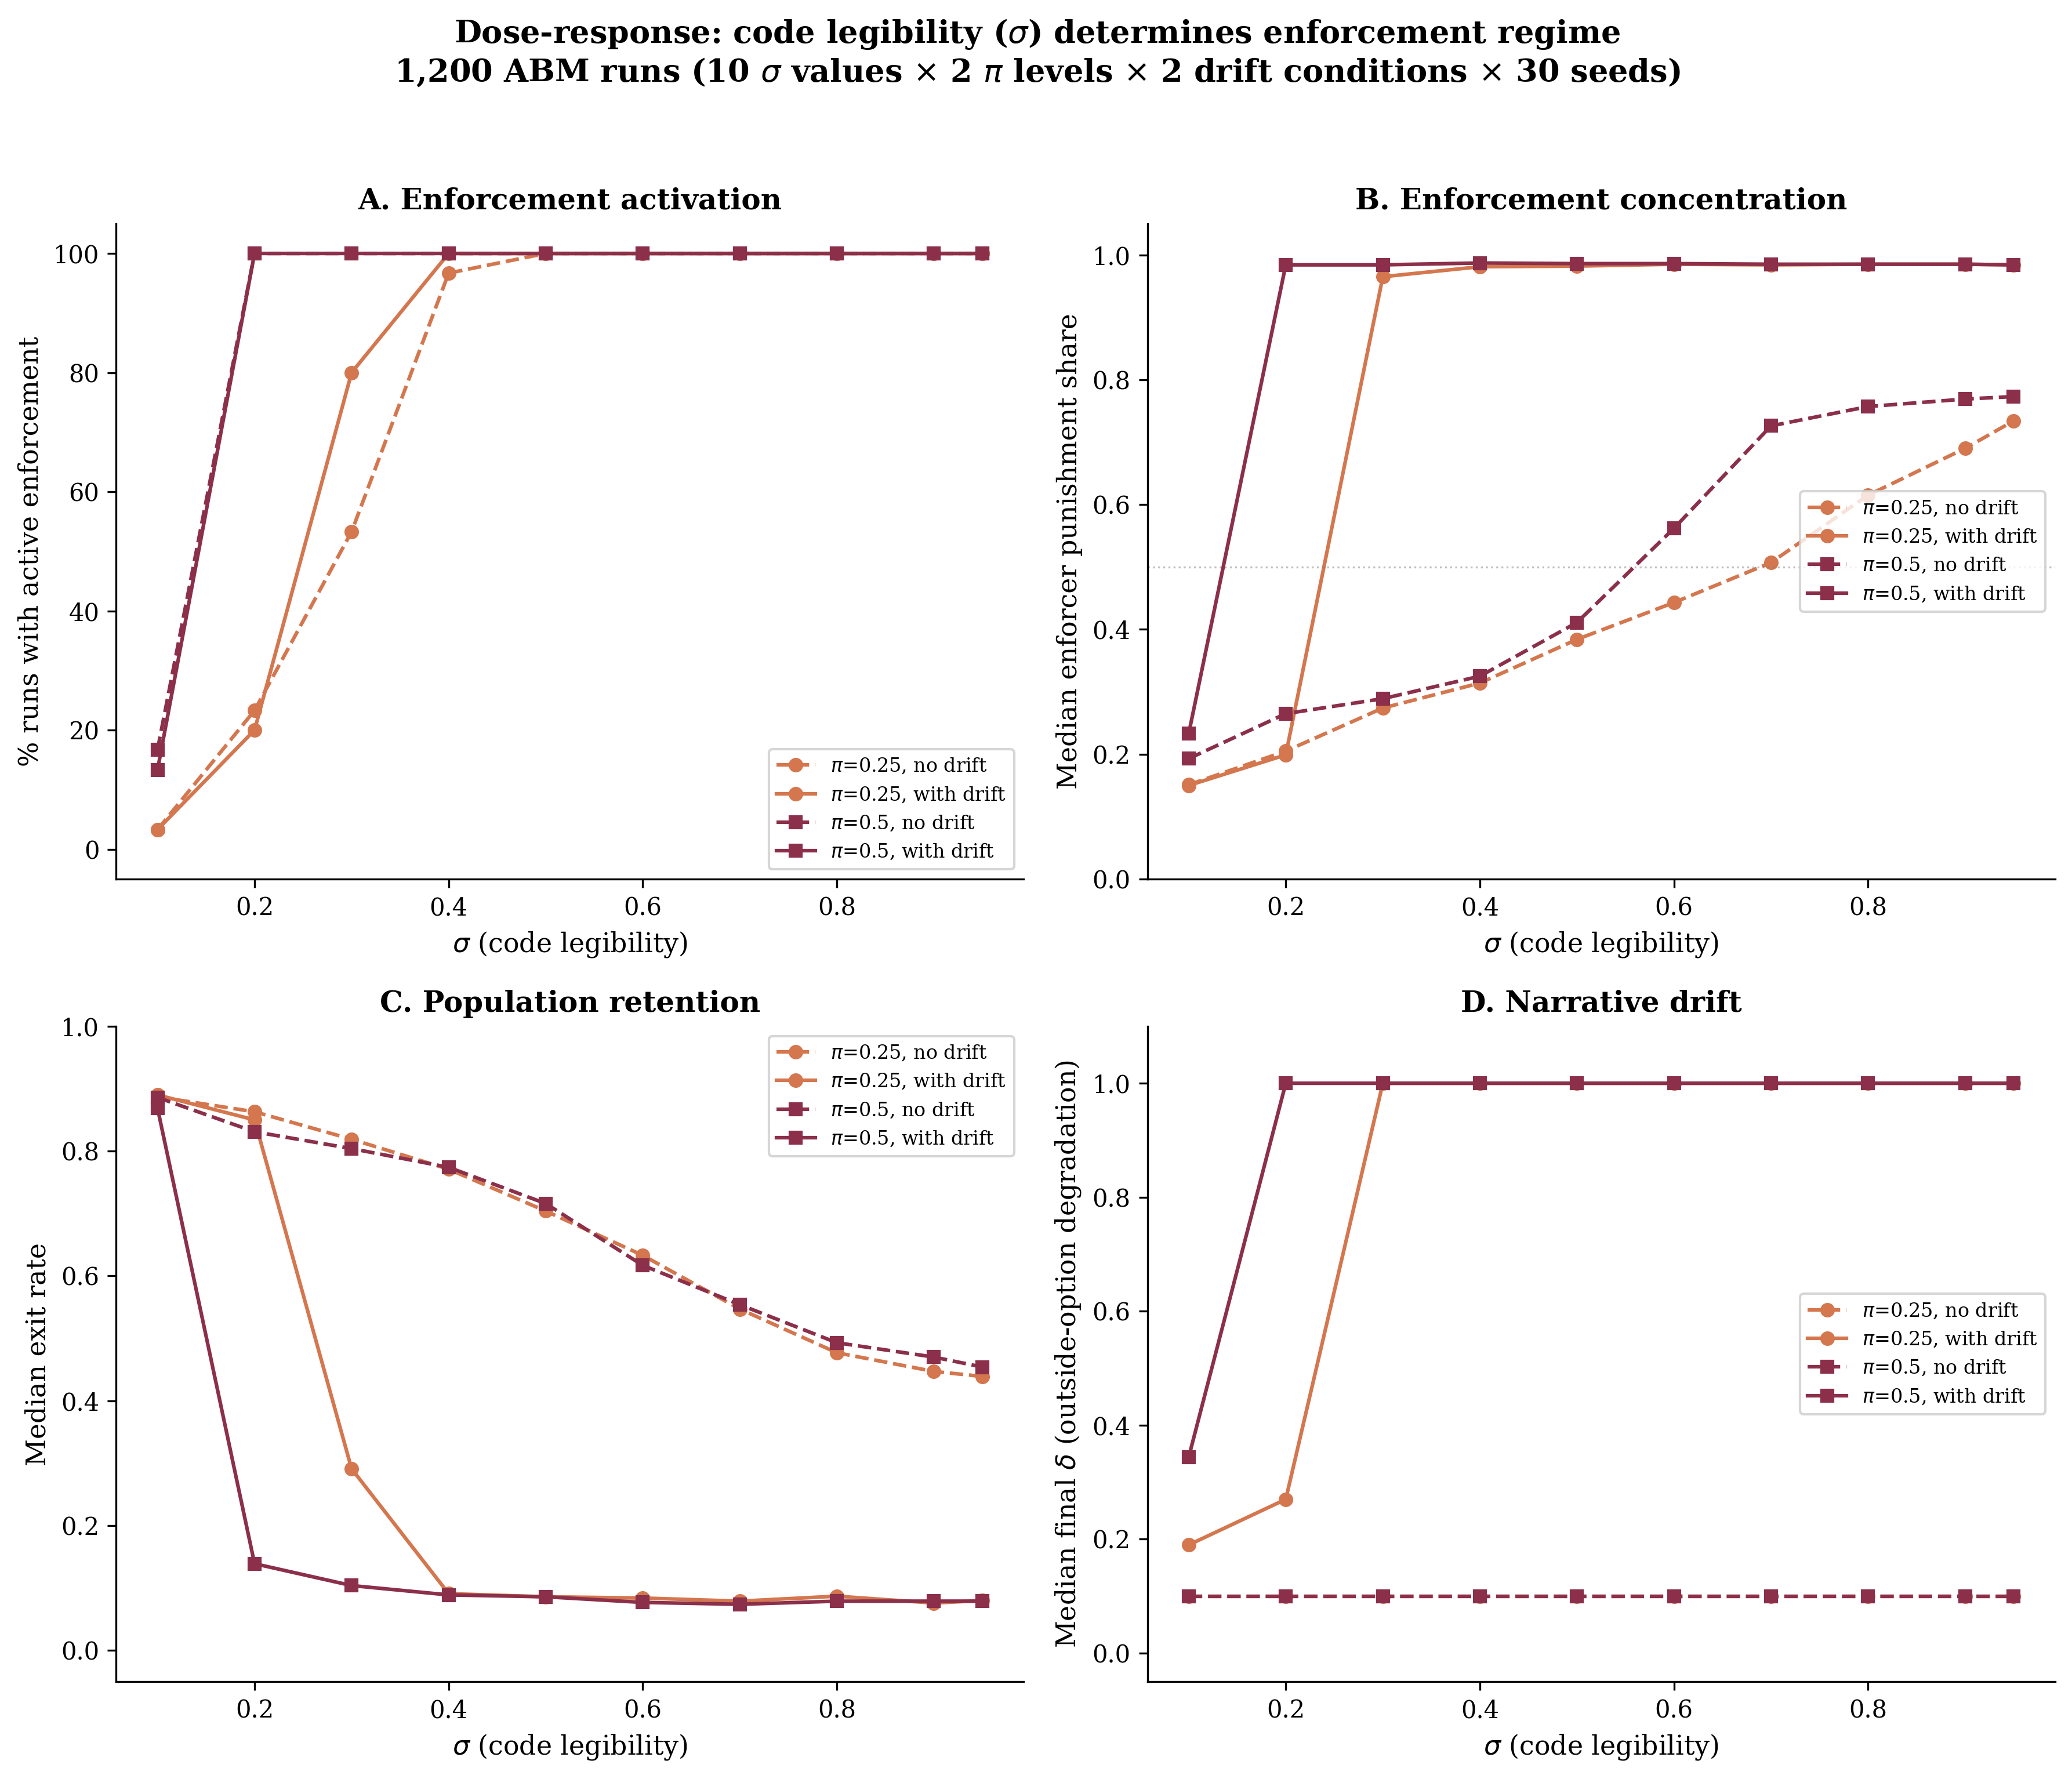
\includegraphics[width=\textwidth]{Fig6}
\caption{Dose-response: code legibility ($\sigma$) determines enforcement regime.
1,200 ABM runs (10 $\sigma$ values $\times$ 2 $\pi$ levels $\times$ 2 drift conditions $\times$ 30 seeds).
Panel A: enforcement activation. Panel B: enforcement concentration (enforcer punishment share).
Panel C: population retention (exit rate). Panel D: narrative drift (final $\delta$).
Solid lines: drift enabled ($\eta = 0.10$). Dashed lines: drift disabled ($\eta = 0$).
Sand/sienna: $\pi = 0.25$. Wine/charcoal: $\pi = 0.50$.}
\end{figure}

\section{Discussion}

%
\subsection{Fundamentalism as structural equilibrium}

The results support the paper's central claim: enforcement-dominant dynamics arise endogenously from the structural properties of codified moral systems, without requiring abnormal psychological distributions, charismatic capture, or exogenous political shocks. The causal chain runs from code geometry (legibility × enforcement reward) through institutional delegation (which concentrates enforcement in a minority) through endogenous narrative drift (which collapses exit) to stable capture. Each link was isolated and confirmed: the y₀ ablation (§8.3) rules out belief convergence as the mechanism; the α and μ null results (§8.5, §8.6) rule out internal retention mechanisms; the η = 0 control (§8.9) rules out initial δ values as the driver. What remains is enforcement economics operating on code structure.

This reframes the standard explanatory sequence. The conventional account treats fundamentalism as a deviation: something goes wrong (extremists infiltrate, a crisis radicalizes, a charismatic leader emerges) and the system is pushed off its natural trajectory. The model indicates that fundamentalism is not a deviation but an available equilibrium state, one that the system will occupy when its structural parameters fall in the appropriate region of parameter space. Removing the "extremists" does not remove the equilibrium. If the code geometry that generated the enforcement niche persists, the niche will be re-occupied.

The practical implication is that interventions targeting individuals (deradicalization programs, leadership decapitation, banning specific organizations) address symptoms rather than structure. The model predicts that such interventions will produce transient disruption followed by reconvergence, because the enforcement niche is a property of the code's geometry, not of the individuals who currently fill it. Structural interventions (reducing legibility, increasing exit feasibility, decentralizing adjudication) act on the parameters that determine which regime the system occupies.

%

\textbf{The two faces of code geometry.}

A consistent finding across all model versions is the decoupling of enforcement production from population retention. The inward-facing dimensions of code geometry (σ, π, delegation, capital compounding) reliably produce enforcement concentration. In every active cell across every sweep, the top 5 agents issue 67 to 92 percent of all punishment and endogenously selected cadre members deliver 92 to 98 percent. This concentration is invariant to retention parameters (α, μ, δ), to drift parameters (η), and to initial conditions. It is a structural consequence of delegation and compounding, not a contingent outcome.

But concentration alone does not produce capture. In the absence of retention mechanisms, the system stabilizes as a mixed regime: enforcement is vigorous and concentrated, but 30 to 40 percent of the population exits. The enforcement apparatus is structurally intact; it simply operates in a community that is hemorrhaging members. This is the regime occupied by most real-world systems with moderate exit costs: active enforcement coexists with substantial attrition.

The transition from mixed to capture requires collapsing the outside option. Of the three candidate mechanisms tested, only alternative degradation achieves this, and only at extreme values (δ ≥ 0.8 for exogenous δ; endogenous drift to δ = 1.0 via the feedback loop). The distinction between inward-facing and outward-facing code geometry reflects a genuine structural asymmetry in how codified systems produce and sustain enforcement.

%

\textbf{What the null results demonstrate.}

The failure of sanctified suffering (α) and membership reward (μ) carries theoretical weight beyond the negative finding itself. Both mechanisms are widely invoked in the sociology of religion and the study of high-control groups. The α mechanism corresponds to a large theological literature on the redemptive value of suffering (from the Christian theology of the cross through the Shi'a veneration of Husayn's martyrdom to the Hasidic doctrine of descent for the sake of ascent). The μ mechanism corresponds to Iannaccone's entire club-goods framework: membership confers benefits that offset the costs of strictness.

Both are real phenomena. Religious communities do reframe discipline as purification, and membership does confer genuine benefits. But neither mechanism produces retention under enforcement pressure when viable alternatives exist. The explanation is structural: both α and μ modify the interior of the payoff comparison (making staying slightly more attractive), while the exit decision is governed by the ratio of inside utility to outside opportunity. Adding a small constant to a large numerator produces negligible change in the ratio. Subtracting from a small denominator produces proportionally large change.

This result has a direct empirical prediction. Communities that employ sanctified-suffering framing or that provide generous membership benefits will not, on the basis of those features alone, achieve lower exit rates than comparable communities without them, once enforcement intensity is controlled for. Retention should correlate with outside-option degradation (geographic isolation, non-transferable human capital, legal apostasy penalties, kinship network closure), not with internal meaning-making or club-goods provision. The club-goods literature predicts that higher membership benefits produce higher retention; the model predicts that membership benefits are inert with respect to retention under enforcement. These predictions are distinguishable in cross-sectional data.

The null results also illuminate why theological content is not a useful predictor of enforcement dynamics. A tradition may possess an elaborate theology of sanctified suffering; it may offer rich communal benefits; it may articulate a sophisticated internal logic for why discipline serves the disciple's interest. None of this matters for retention if the outside option remains viable. The features that matter are prosaic and structural: how hard it is to leave, how degraded the outside appears, how concentrated the enforcement apparatus is. The theological superstructure rides on a structural chassis, and it is the chassis that determines the regime.

%
\subsection{Feedback loop, historical patterns, and existing frameworks}

The endogenous δ drift mechanism captures a dynamic that is extensively documented in the empirical literature on high-control groups but has not previously been formalized. As enforcement concentrates in a specialized minority, that minority gains disproportionate control over community communication channels: sermons, curricula, media, marriage counseling, dispute resolution. This control is exercised not through conspiracy but through institutional incumbency; the same agents who punish also teach, and their institutional position grants them platform access that non-enforcers lack.

The content of their communication shifts the community's perception of the outside world. In Qutb's formulation [33], pre-Islamic ignorance (jahiliyya) is not merely a historical period but a permanent condition of non-Islamic societies, requiring perpetual separation and vigilance. In the Jehovah's Witnesses' doctrinal system, non-members occupy "Satan's world," a characterization reinforced weekly through study materials produced by the Governing Body (the enforcement-and-doctrine apparatus). In Scientology, non-members and former members are classified as "suppressive persons" whose influence is doctrinally toxic. In Soviet ideology, the capitalist world was not merely different but actively decomposing, requiring ideological fortification against contamination [46]. In each case, the enforcement apparatus produces the narrative that degrades the outside option, and the degraded outside option retains the population that sustains the enforcement apparatus. The loop is self-reinforcing.

The model's intensity gate (drift fires only when enforcement exceeds the institutional-salience threshold) captures a second empirical regularity: not all communities with identifiable enforcement roles develop this feedback dynamic. Many religious communities have designated authorities (pastors, rabbis, imams, elders) who exercise mild disciplinary functions without reshaping community cosmology. The gate distinguishes between enforcement that is institutionally present but functionally inert (a pastor who occasionally counsels against gossip) and enforcement that is institutionally dominant (a morality police that patrols public space, adjudicates dress violations, and controls the community's informational environment). Only the latter drives narrative drift. The model reproduces this distinction: quiet cells (max\_punish \textless{} 0.08) show no drift regardless of η, while active cells (max\_punish ≥ 0.09) show sharp δ increases that in most tested configurations saturate near 1.0. The saturation reflects the high enforcer-share values (≥ 0.97) characteristic of delegated enforcement; whether δ saturation translates to capture depends on the remaining parameter configuration (§8.9).

%

\textbf{Historical anchoring.}

The model predicts that codified systems with high legibility, high
enforcement reward, institutional delegation, and restricted exit will
produce enforcement-dominant dynamics through the endogenous feedback
loop. Five extended case analyses (the Inquisition 1231--1834,
post-Reformation confessionalization, the Wahhabi-Saudi system,
Marxism-Leninism, and quiet-regime confirmations from Therav\=ada and
Quaker traditions) are presented in S2 Text. Each case is analyzed in
terms of its code geometry and the observed enforcement dynamics. The
cross-traditional pattern confirms the structural prediction: across the
Inquisition, the Wahhabi-Saudi system, the Soviet party apparatus, and
the CCP discipline system, the same five-element conjunction
appears---legible compliance, positive enforcement reward, institutional
delegation, compounding enforcement capacity, and restricted exit---despite
sharing no doctrinal content. Where this conjunction is absent (forest
monasticism, Quaker meetings), enforcement-dominant dynamics did not
emerge despite demanding normative expectations.


\textbf{Relationship to existing frameworks.}

The results bear on four established theoretical frameworks.

\textbf{Iannaccone's club-goods model} treats strictness as a screening mechanism that selects for committed members and raises the value of club goods. The present model reproduces the screening effect (high σ and π produce communities with elevated compliance), but it identifies a regime transition that the club framework does not formalize: the shift from screening (ex ante selection) to policing (ex post enforcement by a specialized minority). The μ null result (§8.6) is a direct empirical challenge to the club-goods prediction. If membership benefits are the mechanism sustaining strict groups, then increasing μ should increase retention. It does not. The model suggests that the club-goods mechanism operates in the recruitment phase (who joins and who stays initially) but is irrelevant to the retention-under-enforcement dynamic that characterizes high-control groups.

\textbf{Kuran's preference falsification} produces two regimes (stable falsification and revolutionary cascade). The present model produces four: quiet, mixed, collapse, and capture. The critical addition is that the capture regime is stabilized by institutional delegation and compounding capital in a way that prevents cascade even when private dissent is near-universal. Kuran's framework predicts that all falsification equilibria are vulnerable to cascade when a sufficient number of individuals simultaneously reveal their true preferences. The model predicts that cascade requires not merely preference revelation but the dismantling of the enforcement apparatus's institutional infrastructure, its compounding capital, its delegated authority, its control over narrative. This is a harder condition to satisfy than preference revelation alone, and it accounts for the persistence of capture regimes across decades or centuries despite endemic private dissent. The Inquisition operated for over 150 years despite widespread private skepticism; the Soviet system persisted for 70 years despite endemic preference falsification. Cascade, when it came, required not preference revelation but institutional collapse.

\textbf{Taleb's intolerant-minority mechanism} holds that a small, intransigent minority can impose its preferences on a flexible majority through asymmetric stubbornness. The model's literalism enrichment result (Cohen's d ≈ 2.2 for literalism in enforcers versus the general population) confirms that ideological asymmetry does concentrate in the enforcement apparatus. But the y₀ ablation (§8.3) demonstrates that this concentration arises from enforcement economics (delegation + capital), not from preference asymmetry per se. Literalism heterogeneity without delegation does not produce concentration; delegation without literalism heterogeneity does. The intolerant minority is a consequence of institutional selection, not a cause of enforcement dynamics. Taleb's mechanism may operate in consumer-goods contexts (where kosher certification dynamics have the structure he describes) but does not explain enforcement capture in codified moral systems, where the enforcement apparatus is institutionally constructed rather than emerging from preference rigidity alone.

\textbf{Scott's legibility concept} provides the theoretical foundation for the σ parameter, but the model extends it in a direction Scott did not pursue. Scott analyzed legibility as a property of state-society relations: states simplify and standardize populations to render them administratively governable. The model applies the same logic to intra-community moral governance: codified systems simplify and standardize moral quality to render members doctrinally governable. The extension is not trivial because it operates at a different institutional scale (community rather than state) and addresses a different form of legibility (moral rather than administrative). But the structural logic is identical: legibility enables monitoring, monitoring enables enforcement, enforcement enables control.

%
\subsection{Scope and limitations}

The model omits several features of real codified systems that could alter the dynamics in ways not captured here.

Network structure is treated as a static small-world graph. In real systems, enforcement produces network reconfiguration: enforcers accumulate preferential connections, dissidents are isolated, and boundary-crossing ties (friendships with outsiders, mixed marriages, secular education) are actively severed by the enforcement apparatus. Code-prescribed social boundary rules (endogamy requirements, residential segregation, prohibitions on external media) constitute a distinct mechanism of exit-cost manipulation that operates through network topology rather than through payoff modification. This mechanism requires agent-level network dynamics and is reserved for a companion paper.

Membership benefit is homogeneous across agents. In reality, membership value varies with economic dependence, kinship density, social position, and accumulated community-specific capital. Agents with high community embeddedness face qualitatively different exit calculations than peripheral members. This heterogeneity could produce differential exit (peripheral members leave first, embedded members remain) and compositional effects (the retained population is disproportionately embedded, which increases mean exit cost endogenously). The model's homogeneous μ likely underestimates retention in the intermediate δ range.

The model does not include exogenous shocks (political crises, external threats, modernization pressures) that figure prominently in empirical accounts of fundamentalist mobilization [1]. The framework treats such shocks as parameter perturbations (a crisis increases π or reduces base\_opp) rather than as independent causal mechanisms: it identifies the structural substrate on which shocks operate, not the shocks themselves. But it means that the model cannot account for the timing of fundamentalist episodes, only for the structural conditions that make them possible.

The intensity gate on δ drift introduces a researcher-specified threshold (punish\_floor = 0.08). The calibration is empirically grounded (it tracks the quiet-to-active boundary observed in the baseline sweep), but the specific value is a modeling choice. Sensitivity analysis (not reported here) indicates that the qualitative results are preserved for floor values between 0.06 and 0.12; outside this range, the gate is either too permissive (drift in quiet cells) or too restrictive (blocking drift in clearly active cells).

%

\subsection{Empirical consistency}

The framework generates predictions testable against cross-national and
within-US data. These tests are exploratory; the sample sizes and proxy
measures do not support causal inference.

\textbf{Cross-national.} We merged RAS Round 3 religious legislation
scores [15] with World Values Survey importance-of-god scores and World
Bank GDP per capita (constant 2015 USD; log-transformed) for 36
countries with complete data. In the combined model ($R^2 = 0.73$), both
log GDP ($\beta = -1.65$, $p < 0.001$; HC3 robust standard errors) and
religious legislation ($\beta = 0.045$, $p = 0.027$) independently
predict religious retention. A bootstrap analysis (10,000 resamples)
yields a median $R^2$ ratio (GDP model / legislation model) of 1.18 with
95\% CI $[0.64, 2.18]$. The confidence interval includes 1.0; the
sample is underpowered (post hoc power = 0.18) to rank the predictors'
relative contributions. Both matter.

\textbf{Within-US.} Pew retention data for 15 US religious groups
complicates the picture. Club-goods provision correlates with retention
($\rho = 0.72$, $p = 0.002$), but ethno-cultural identity confounds the
association ($\rho = 0.86$ with retention, $\rho = 0.55$ with
club-goods). In a four-variable model ($R^2 = 0.92$), ethno-cultural
identity dominates ($\beta = 7.73$, $p < 0.001$); outside-option
degradation does not reach significance ($p = 0.08$). The most
informative comparison: Jehovah's Witnesses and Scientology score highest
on enforcement intensity and outside-option degradation narratives, yet
retain the fewest members (34\% and 30\%). The Amish, with equivalent
narrative scores, retain 85\%. The difference is structural: Amish exit
barriers (geographic isolation, non-transferable skills, 8th-grade
terminal education) degrade the actual outside option; JW and Scientology
barriers (shunning, disconnection) raise emotional costs without
eliminating the option. This maps to the model's $\delta$: retention
under enforcement tracks structural exit barriers, not narrative ones.

\subsection{Authority architecture and the legibility gradient}

The dose-response curve identifies a structural boundary separating the
quiet region from enforcement-dominant dynamics. This boundary has a
theoretical interpretation connecting the computational result to how
codified systems structure the relationship between truth and persons.

In transpersonal authority systems, truth is located outside any person's
biography. The Vedic tradition's doctrine of \emph{apaurusheya}
(authorlessness) is the most fully articulated instance: the Vedas are
\emph{nitya} (eternal), no person authored them, and the \emph{rishi}s
are seers, not makers. When truth has no author, moral evaluation cannot
terminate at external behavior because the tradition denies that external
performance constitutes the relevant epistemic achievement. $\sigma$ is
structurally low. The enforcement niche cannot form. (For a detailed
philosophical analysis of transpersonal authority and its institutional
consequences across six comparison cases, see Boggavarapu, forthcoming.)

In person-dependent authority systems, truth arrives through a specific
individual's biography. Compliance becomes adherence to the messenger's
codified prescriptions, which are necessarily external, behavioral, and
legible. $\sigma$ is structurally high. The model predicts active
dynamics at $\sigma \geq 0.4$, and every tested configuration above this
threshold produces enforcement concentration.

The intermediate zone ($\sigma = 0.2$--$0.3$) maps to traditions with
hybrid authority architectures. Buddhist practice is person-independent
in stated intent but tethered to a specific biography. The model
reproduces this variability: at $\sigma = 0.3$, $\pi = 0.25$, 80\% of
seeds activate but 20\% remain quiet.

The connection is structural, not analogical. Person-dependent authority
produces legible compliance as a logical consequence: if truth comes
through a person, adherence to that person's rules is the criterion of
standing, and rules are observable. Transpersonal authority produces
opaque compliance: if truth belongs to no person, realization rather than
performance is the criterion, and realization is unobservable.

This analysis does not claim that named traditions are fixed at specific
$\sigma$ values. A single tradition traverses different regions of
parameter space as institutional conditions change. Ottoman Sufi tariqas
and Taliban Afghanistan are both ``Islamic'' but occupy different code
geometries. The scoring unit is the regime, not the tradition.



The model claims that fundamentalism, understood as enforcement-dominant dynamics in codified moral systems, is a structural equilibrium rather than an exogenous pathology. It claims that the transition to this equilibrium depends on code geometry (legibility, enforcement reward, delegation, capital compounding) and on the endogenous degradation of the outside option by the enforcement apparatus. It claims that internal retention mechanisms (sanctified suffering, membership rewards) are insufficient for capture in the presence of viable alternatives. And it claims that the feedback loop from enforcement concentration to narrative drift to retention is the mechanism that stabilizes the capture regime.

The model does not claim that all religious enforcement is pathological. The quiet and mixed regimes are structurally normal features of codified systems. Enforcement exists in every community that maintains behavioral standards; concentration exists wherever institutional delegation occurs. The model identifies the specific conditions under which these generic features become self-reinforcing to the point of capture, and those conditions require an additional mechanism (endogenous outside-option degradation) that most systems do not activate.

The model does not claim that theology is irrelevant. Theological content determines many features of lived religious experience that the model does not address: meaning, identity, community formation, ethical development, aesthetic practice. The claim is narrower: theological content does not determine enforcement regime type. Two traditions with identical code geometry but different theological commitments are predicted to exhibit similar enforcement dynamics. Whether this prediction holds empirically is a testable question, and falsification would require revision of the framework's central assumption.

The model does not claim that fundamentalism is inevitable for all codified systems. It predicts that systems whose code geometry falls in the active region of parameter space (sufficient legibility, sufficient enforcement reward, institutional delegation, compounding capital) will generate enforcement-dominant dynamics through the endogenous feedback loop. The prediction is conditional on parameter values, not on contingent historical events. Whether a specific real-world system occupies the capture region depends on measurable structural features of its code and institutions; the model's contribution is to identify which features determine the outcome. The uncertainty is in parameter measurement, not in the dynamics.

%
\section{Conclusions}

Enforcement-dominant equilibria in codified moral systems arise from
the information-theoretic properties of the code, not from the content
of belief. Code geometry determines whether monitoring is feasible;
feasible monitoring activates enforcement; institutional delegation
concentrates enforcement in an endogenously selected minority;
concentrated enforcement drives narrative degradation of the outside
world; degraded outside options suppress exit; suppressed exit stabilizes
the enforcement apparatus. Each link was isolated through ablation.
Removing the institutional monopoly restriction leaves concentration
unchanged (top-5 share: 0.81--0.90 in both conditions; 180 matched runs).
Sanctified suffering and membership reward are inert across their full
parameter ranges. Only degradation of the outside option closes the
feedback loop.

The dose-response analysis identifies the structural boundary. Below the
activation threshold, enforcement cannot engage: the code is too opaque
for monitoring. Above the boundary (whose position shifts with $\pi$:
near $\sigma = 0.3$ at moderate reward, $\sigma = 0.2$ at high reward),
enforcement activates, concentrates, and with narrative drift collapses
exit. Legibility is the gate. Enforcement reward shifts the boundary.
Endogenous narrative drift closes the trap.

This boundary corresponds to how codified systems relate truth to
persons. Transpersonal authority produces low $\sigma$ as a logical
consequence and occupies the quiet region. Person-dependent authority
produces high $\sigma$ and occupies the active region. The model predicts
that enforcement regime type correlates with code-geometry scores rather
than with theological strictness or doctrinal conservatism. The
Inquisition, the Wahhabi enforcement apparatus, Marxist-Leninist party
discipline, and post-Reformation confessionalization instantiate the same
structural pattern despite sharing no doctrinal content. Where the
conjunction of legible compliance, enforcement reward, institutional
delegation, and restricted exit is present, enforcement-dominant dynamics
emerge. Where it is absent, they do not.

Three limitations bound the result. The model uses a static network.
Membership benefit is homogeneous. The cross-national analysis is
exploratory and underpowered ($N = 36$; power = 0.18). Planned tests
against the Religion and State Dataset, Inquisition prosecution records,
and Religious Landscape Studies panel data would provide stronger causal
identification.

The claim is conditional. The quiet regime occupies the largest region of
parameter space. When enforcement-dominant dynamics appear, they arise
from measurable structural properties independent of what the code says.
The dose-response curve maps that region with precision.

\section*{Data Availability Statement}

All simulation source code, parameter configurations, analysis scripts,
and ablation experiment scripts are available at [repository URL].
Supporting data: S1 Data (baseline sweep summary), S2 Data (seed-level
results), S3 Data (monopoly ablation comparison), S4 Data (cadre quota
sensitivity), S5 Data (intensity gate sensitivity), S6 Data
(dose-response sweep, 1,200 runs), S7 Data (cross-national regression
with bootstrap analysis). The Religion and State Dataset Round 3 is
available from the Association of Religion Data Archives. World Values
Survey data from the World Values Survey Association. World Bank GDP data
from the World Bank Open Data portal.

\section*{Competing Interests}

The author declares no competing interests.

%
\section*{Author Contributions}

Conceptualization: [Author Name]. Formal analysis: [Author Name]. Investigation: [Author Name]. Methodology: [Author Name]. Software: [Author Name]. Visualization: [Author Name]. Writing, original draft: [Author Name]. Writing, review and editing: [Author Name].

%
\section*{Supporting Information}

S1 Data. Sweep summary statistics. Cell-level median metrics and regime classifications for the exploratory parameter sweep (108 cells, 216 runs). (CSV)

S2 Data. Seed-level results. Individual run metrics and regime classifications for all exploratory sweep runs. (CSV)

S1 Text. Extended model specification. Complete parameter table, sensitivity analysis for regime classification thresholds, and intensity gate calibration details.

S1 Table. Within-US retention analysis. Full scoring rubric and dataset for 15 US religious groups on outside-option degradation, club-goods provision, enforcement intensity, and ethno-cultural identity components.

S1 Fig. Exploratory sweep phase maps. Phase map from the initial 108-cell exploratory sweep (2 seeds per cell) showing regime boundary structure prior to confirmatory analysis.

%
\section*{References}

\begin{enumerate}
\def\labelenumi{\arabic{enumi}.}
\item
  Almond, G. A., Appleby, R. S., \& Sivan, E. (2003). \emph{Strong Religion: The Rise of Fundamentalisms around the World}. University of Chicago Press.
\item
  Axelrod, R. (1986). An evolutionary approach to norms. \emph{American Political Science Review}, 80(4), 1095--1111.
\item
  Berman, E. (2000). Sect, subsidy, and sacrifice: An economist's view of ultra-Orthodox Jews. \emph{Quarterly Journal of Economics}, 115(3), 905--953.
\item
  Berman, E., \& Laitin, D. D. (2008). Religion, terrorism and public goods: Testing the club model. \emph{Journal of Public Economics}, 92(10--11), 1942--1967.
\item
  Boyd, R., Gintis, H., Bowles, S., \& Richerson, P. J. (2003). The evolution of altruistic punishment. \emph{Proceedings of the National Academy of Sciences}, 100(6), 3531--3535.
\item
  Bromley, D. G. (Ed.). (1998). \emph{The Politics of Religious Apostasy: The Role of Apostates in the Transformation of Religious Movements}. Praeger.
\item
  Carvalho, J.-P. (2013). Veiling. \emph{Quarterly Journal of Economics}, 128(1), 337--370.
\item
  Centola, D., Willer, R., \& Latan, M. (2005). The emperor's dilemma: A computational model of self-enforcing norms. \emph{American Journal of Sociology}, 110(4), 1009--1040.
\item
  Cohen, A. B., \& Rozin, P. (2001). Religion and the morality of mentality. \emph{Journal of Personality and Social Psychology}, 81(4), 697--710.
\item
  Cook, M. (2000). \emph{Commanding Right and Forbidding Wrong in Islamic Thought}. Cambridge University Press.
\item
  Cragun, R. T., \& Hammer, J. H. (2011). "One person's apostate is another person's convert": What terminology tells us about pro-religious hegemony in the sociology of religion. \emph{Humanity \& Society}, 35(1--2), 149--175.
\item
  Fehr, E., \& Gächter, S. (2000). Cooperation and punishment in public goods experiments. \emph{American Economic Review}, 90(4), 980--994.
\item
  Fehr, E., \& Gächter, S. (2002). Altruistic punishment in humans. \emph{Nature}, 415(6868), 137--140.
\item
  Fitzpatrick, S. (2005). \emph{Tear Off the Masks! Identity and Imposture in Twentieth-Century Russia}. Princeton University Press.
\item
  Fox, J. (2019). \emph{The Religion and State Project}, Round 3. Association of Religion Data Archives.
\item
  Gelfand, M. J., et al.~(2011). Differences between tight and loose cultures: A 33-nation study. \emph{Science}, 332(6033), 1100--1104.
\item
  Given, J. B. (1997). \emph{Inquisition and Medieval Society: Power, Discipline, and Resistance in Languedoc}. Cornell University Press.
\item
  Greif, A. (2006). \emph{Institutions and the Path to the Modern Economy: Lessons from Medieval Trade}. Cambridge University Press.
\item
  Greif, A., \& Mokyr, J. (2016). Cognitive rules, institutions, and economic growth: Douglass North and beyond. \emph{Journal of Institutional Economics}, 13(1), 25--52.
\item
  Hilbe, C., Traulsen, A., Röhl, T., \& Milinski, M. (2014). Democratic decisions establish stable authorities that overcome the paradox of second-order punishment. \emph{Proceedings of the National Academy of Sciences}, 111(2), 752--756.
\item
  Hirschman, A. O. (1970). \emph{Exit, Voice, and Loyalty: Responses to Decline in Firms, Organizations, and States}. Harvard University Press.
\item
  Hagberg, A. A., Schult, D. A., \& Swart, P. J. (2008). Exploring network structure, dynamics, and function using NetworkX. In \emph{Proceedings of the 7th Python in Science Conference} (pp.~11--15).
\item
  Iannaccone, L. R. (1992). Sacrifice and stigma: Reducing free-riding in cults, communes, and other collectives. \emph{Journal of Political Economy}, 100(2), 271--291.
\item
  Iannaccone, L. R. (1994). Why strict churches are strong. \emph{American Journal of Sociology}, 99(5), 1180--1211.
\item
  Kelly, H. A. (1989). Inquisition and the prosecution of heresy: Misconceptions and abuses. \emph{Church History}, 58(4), 439--451.
\item
  Kazil, J., Masad, D., \& Crooks, A. (2020). Utilizing Python for agent-based modeling: The Mesa framework. In \emph{Social, Cultural, and Behavioral Modeling} (pp.~308--317). Springer.
\item
  Kotkin, S. (1995). \emph{Magnetic Mountain: Stalinism as a Civilization}. University of California Press.
\item
  Kuran, T. (1995). \emph{Private Truths, Public Lies: The Social Consequences of Preference Falsification}. Harvard University Press.
\item
  Mann, M. (1986). \emph{The Sources of Social Power}, Vol. 1. Cambridge University Press.
\item
  Norenzayan, A., \& Gervais, W. M. (2013). The origins of religious disbelief. \emph{Trends in Cognitive Sciences}, 17(1), 20--25.
\item
  North, D. C. (1990). \emph{Institutions, Institutional Change and Economic Performance}. Cambridge University Press.
\item
  Pierson, P. (2000). Increasing returns, path dependence, and the study of politics. \emph{American Political Science Review}, 94(2), 251--267.
\item
  Qutb, S. (1964). \emph{Milestones} [\emph{Ma'alim fi al-Tariq}]. Various editions.
\item
  Reinhard, W. (1983). Zwang zur Konfessionalisierung? Prolegomena zu einer Theorie des konfessionellen Zeitalters. \emph{Zeitschrift für historische Forschung}, 10(3), 257--277.
\item
  Rubin, J. (2017). \emph{Rulers, Religion, and Riches: Why the West Got Rich and the Middle East Did Not}. Cambridge University Press.
\item
  Schilling, H. (1988). Die Konfessionalisierung im Reich: Religiöser und gesellschaftlicher Wandel in Deutschland zwischen 1555 und 1620. \emph{Historische Zeitschrift}, 246(1), 1--45.
\item
  Scott, J. C. (1998). \emph{Seeing Like a State: How Certain Schemes to Improve the Human Condition Have Failed}. Yale University Press.
\item
  Sigmund, K., De Silva, H., Traulsen, A., \& Hauert, C. (2010). Social learning promotes institutions for governing the commons. \emph{Nature}, 466(7308), 861--863.
\item
  Streib, H., Hood, R. W., Keller, B., Csöff, R.-M., \& Silver, C. F. (2009). \emph{Deconversion: Qualitative and Quantitative Results from Cross-Cultural Research in Germany and the United States of America}. Vandenhoeck \& Ruprecht.
\item
  Taleb, N. N. (2018). \emph{Skin in the Game: Hidden Asymmetries in Daily Life}. Random House.
\item
  Tilly, C. (1985). War making and state making as organized crime. In P. Evans, D. Rueschemeyer, \& T. Skocpol (Eds.), \emph{Bringing the State Back In} (pp.~169--191). Cambridge University Press.
\item
  Ulmer, J. T., Bader, C., \& Gault, M. (2008). Do moral communities play a role in criminal sentencing? Evidence from Pennsylvania. \emph{Sociological Quarterly}, 49(4), 737--768.
\item
  Wedeen, L. (1999). \emph{Ambiguities of Domination: Politics, Rhetoric, and Symbols in Contemporary Syria}. University of Chicago Press.
\item
  Watts, D. J., \& Strogatz, S. H. (1998). Collective dynamics of `small-world' networks. \emph{Nature}, 393(6684), 440--442.
\item
  Weber, M. (1919/1946). Politics as a Vocation. In H. H. Gerth \& C. W. Mills (Eds.), \emph{From Max Weber: Essays in Sociology} (pp.~77--128). Oxford University Press.
\item
  Yurchak, A. (2005). \emph{Everything Was Forever, Until It Was No More: The Last Soviet Generation}. Princeton University Press.
\end{enumerate}

\end{document}
